\chapter{Wprowadzenie teoretyczne}\label{cha:czescTeoretyczna}

	\section{Przegląd drzew \emph{Trie}}\label{sec:czescTeoretycznaPrzegladDrzewTrie}
	
		Oprócz artykułów na różnych stronach internetowych, w literaturze naukowej można znaleźć wiele terminów czy opisów zawierających hasło \emph{Trie}. Przykładem takiego źródła jest znana wszystkich książka Cormen'a (i innych) ``Wprowadzenie do algorytmów``~\cite{CormensIntroductionToAlgorithms}, posiadająca pod-rozdział o tytule ``y-fast tries`` nawiązujący do drzew van Emde Boas'a. Zdecydowanie trudniej znaleźć publikacje, które rozlegle i dogłębnie omawiają termin ,,zwykłego`` drzewa \emph{Trie} i \emph{Patricia}. Na szczęście istnieje dzieło Donalda Knuth'a o nazwie ``Sztuka programowania``, a w szczególności tom 3~\cite{KnuthsTheArtOfComputerProgramming3}, w którym można znaleźć cały rozdział poświęcony terminowi \emph{Trie} i \emph{Patricia}.
	
		\subsection{Historia terminu \emph{Trie}}\label{sec:czescTeoretycznaPrzegladDrzewTrieHistoriaTerminuTrie}
    	Po raz pierwszy drzewo \emph{Trie} zostało przedstawione przez Axel Thue jako abstrakcyjne pojęcie użyte do reprezentacji zbioru ciągów znaków. W pracy o ``Ciągach znaków niezawierających przyległych powtarzających się podciągów znaków``~\cite{ThuesSelectedMathematicalPapers} z 1912 roku Axel zaprezentował implementację przy użyciu tablicy o rozmiarze rozważanego alfabetu.
		
		Pamięć typu \emph{Trie} w kontekście przeszukiwania komputerowego została szerzej opisana przez René de la Briandais w artykule ``Przeszukiwanie pliku używając kluczy o~zmiennej długości`` z roku 1959~\cite{BriandaisWesternJointComputerConf,MediumComTryingToUnderstandTries}. René zauważył, że korzystając z listy zamiast tablic, oszczędzimy pamięć kosztem czasu wykonywania.
				
		Termin \emph{Trie} został użyty dopiero w 1960 roku przez Edwarda Fredkina w artykule ``Trie Memory``~\cite{FredkinsTrieMemory}. Nazewnictwo to zostało zaczerpnięte z wyrażenia angielskiego \emph{information retrieval}, które oznacza wyszukiwanie informacji. Wymowę terminu \emph{Trie} zmodyfikowano na odpowiadającą słowu \emph{try} na potrzeby odróżnienia go od wymowy \emph{tree}.
	
		\subsection{Struktura i definicja}\label{sec:czescTeoretycznaPrzegladDrzewTrieStruktura}	
		Donald E. Knuth w swoim trzecim tomie książki pod tytułem ``Sztuka Programowania``~\cite{KnuthsTheArtOfComputerProgramming3} wymienia wspomniane oraz inne abstrakcyjne konstrukcje kryjące się pod terminem \emph{Trie}.
		
		Zgodnie z jego definicją \emph{Trie} to drzewo posiadające węzły o co najwyżej $M$ dzieciach. To tak zwane drzewo \emph{M-ary} \cite{wikiMAry} lub \emph{M-way} tłumaczone jako drzewo stopnia $M$. Oczywiście zamiast litery $M$ w nazwie takiego drzewa mogą zostać użyte inne litery, na przykład $N$ lub $K$. 
		
		Oprócz tego, węzły drzewa \emph{Trie} mają postać $M$-elementowych wektorów. Komórki tych wektorów są przyporządkowane znakom, na przykład pojedynczym literom bądź cyfrom. 
		
		Każdy znak pozwala na przejście gałęzią z jednego węzła znajdującego się na poziomie $L$ do następnego węzła znajdującego się na poziomie $L+1$, gdzie korzeń drzewa odpowiada pustej sekwencji znaków i jest na poziomie $0$. Węzeł na poziomie $L$ reprezentuje ostatni element sekwencji znaków o długości $L$, która jest nazywana prefiksem omawianego węzła. Prefiks niekoniecznie musi być całym słowem znajdującym się w drzewie \emph{Trie}, a jedynie jego fragmentem. Węzeł na każdym poziomie posiada M rozgałęzień - wychodzących krawędzi - prowadzących na poziom $L+1$. Elementem decydującym, którą gałąź należy wybrać, jest znak w sekwencji o numerze $L+1$. 
	
        Należy zwrócić uwagę na to, że Knuth definiuje poziom węzła~\cite{KnuthsTheArtOfComputerProgramming1} w sposób rekursywny, gdzie korzeń drzewa znajduje się na poziomie $L = 0$, a poziom innych węzłów jest równy odległości liczonej w krawędziach od korzenia do danego, omawianego węzła. Taki mały szczegół może przyprawić czytelnika o poważny ból głowy.
		
    	Do każdego z tych dzieci można się dostać poprzez jeden z zestawu kluczy reprezentowanych przez węzeł rodzica. Inaczej mówiąc, węzeł rodzic jest rozgałęzieniem drzewa na $M$ węzłów dzieci -- stąd nazwa \emph{M-way}, bo posiada $M$ dróg wychodzących. Efektem tego założenia jest zależność położenia każdego z węzłów dzieci od sekwencji znaków o~długości $L+1$. Prawdziwe jest też stwierdzenie, że położenie węzła dziecka względem węzła rodzica jest określane przez element ciągu znaków o numerze $L+1$.
    	
    	Szczególnie popularną wariacją drzewa \emph{Trie} ze względu na mylącą prostotę rozwinięcia jego koncepcji jest drzewo \emph{Patricia}. Na pytanie na czym polega ta koncepcja oraz o tym czy jest ona rzeczywiście prosta do zastosowania w praktyce odpowiadam w~sekcji dotyczącej drzewa \emph{Patricia}~\ref{sec:DrzewoPatricia}.
		
	\ifsourcematerial
		\begin{displayquote}
			\color{ao(english)}
			\underline{\textbf{FRAGMENT TŁUMACZONY:}} \newline
			A trie \elide is essentially an \emph{M-ary} tree, whose nodes are \emph{M-place} vectors with components corresponding to digits or characters. Each node on level \emph{l} represents the set of all keys that begin with a certain sequence of \emph{l} characters called \textbf{its prefix;} the node specifies an \emph{M-way} branch, depending on the \emph{(l + 1)st} character.
		\end{displayquote}
	\fi
	
        \subsection{Zastosowania praktyczne}\label{sec:ZastosowaniaPraktyczne}
        
        Hasło \emph{Trie} przewija się często w pracach naukowych oraz rozwiązaniach komercyjnych. Przykładami takich zastosowań są:
        \begin{enumerate}
            \item Zastosowania naukowe:
            \begin{enumerate}
                \item Operacje na zbiorach oparte o \emph{Trie} i selektywna komputacja prostych implikantów (ang. ,,\emph{Tri-Based Set Operations and Selective Computation of Prime Implicates}``)~\cite{TriBasedSetOperationsAndSelectiveComputationsOfPrimeImplicates},
                    \subitem Wykorzystanie implikantów prostych do uproszczenia formuł logicznych w formach \emph{CNF} i \emph{DNF};
                \item Rozwiązania dużych problemów wyłuskiwania informacji (ang. ,,\emph{large information-retrieval problems}``)~\cite{PatriciaDonaldRMorrison};
                \item Trie wykorzystujące pliki dla urządzeń wbudowanych (ang. ,,\emph{File Based Trie for Embedded Devices}``)~\cite{FileBasedTrieForEmbeddedDevices};
                \item Samo-stabilizujące się \emph{hash}owe drzewo \emph{Patricia Trie} (ang. \emph{A Self-Stabilizing Hashed Patricia Trie})~\cite{knollmann2018selfstabilizing}.
            \end{enumerate}
            \item Zastosowania komercyjne:
            \begin{enumerate}
                \item Programy w języku Fortran dla komputerów CDC-3600 i UNIVAC 1108~\cite{PatriciaDonaldRMorrison};
                \item Funkcja \emph{Speed Dial} w przeglądarce \emph{Opera};
                \item Słownik T9 na wielu urządzeniach mobilnych.
            \end{enumerate}
            \item Możliwe inne zastosowania:
            \begin{enumerate}
                \item Tablica routingu IPv4;
                \item Sprawdzanie poprawności pisowni;
                \item System podpowiedzi pełnego hasła na podstawie już wpisanego tekstu (ang. \emph{autocomplete}).
            \end{enumerate}
        \end{enumerate}

		\subsection{Przegląd operacji}\label{sec:czescTeoretycznaPrzegladDrzewTrieOperacje}
		
		Keith Schwarz z uniwersytetu Stanford w swoich wykładach~\cite{stanfordKeithSchwarz} przeznaczonych dla kursu dotyczącego struktur danych porusza temat operacji wykonywanych na drzewach, które pełnią funkcję słowników.
		
		Każdy rodzaj drzewa \emph{Trie} lub \emph{Patricia} można postrzegać jako słownik z określoną kolejnością (ang. \emph{ordered dictionary}), który zawiera zbiór $S$ składający się z elementów na płaszczyźnie $U$, która również ma swoją, określoną kolejność (ang. \emph{ordered universe}).
		
        Aby drzewo mogło zostać użyte do przedstawienia takiego słownika, powinno wspierać operacje przedstawione w tym podrozdziale.
        
		\ifsourcematerial
		\begin{displayquote}
			\color{ao(english)}
			\underline{\textbf{FRAGMENT TŁUMACZONY:}} \newline
			
		An ordered dictionary is a data structure that
		maintains a set S of elements drawn from an ordered
		universe U and supports these operations:
		
		\end{displayquote}
		\fi
		
		\subsubsection{Wstaw}\label{sec:czescTeoretycznaPrzegladDrzewTrieOperacjeInsertWstaw}
		
		Operacja wstaw (ang. \emph{insert}) dodaje element $x$, który jest argumentem metody do zbioru $S$. W kontekście drzew \emph{Trie} oraz \emph{Patricia} należy interpretować tę metodę jako dodanie do nich nowego klucza.
		
		\subsubsection{Jest-pusty}\label{sec:czescTeoretycznaPrzegladDrzewTrieOperacjeIsEmptyJestPusty}
		
		Operacja jest-pusty (ang. \emph{is-empty}) odpowiada na pytanie, które może być interpretowane jako:
		
		\begin{itemize}
			\item Czy zbiór $S$ jest pusty ($S=\varnothing$)?
			\item Czy drzewo jest puste? 
			\item Czy struktura posiada dowiązanie (np. wskaźnik) na zainicjowany węzeł, reprezentującym jakiś klucz? W kontekście niektórych algorytmów opisanych w~tym rozdziale dotyczących drzew \emph{Trie} węzeł ten musi być oddzielnym węzłem od korzenia drzewa, a w kontekście pozostałych już sam korzeń drzewa może zawierać informacje na temat klucza.
		\end{itemize} 
		
		Wnioskiem płynącym z tego stwierdzenia jest fakt, że nie każda operacja może być zdefiniowana tylko ze względu na budowę danego rodzaju drzewa \emph{Trie}, czy tylko na charakterystykę kluczy. Jest to spowodowane tym, iż pewne operacje dostarczają cenne informacje dopiero po dobraniu odpowiedniej implementacji do danej budowy drzewa.
		
		\subsubsection{Prefiks}\label{sec:czescTeoretycznaPrzegladDrzewTrieOperacjePrefix}
		
		Operacje dotyczące prefiksów (ang. \emph{prefix}) są metodami odpowiadającymi na pytania dotyczące początkowych fragmentów kluczy zawartych w drzewie, względem słowa będącego argumentem operacji. Prefiksem może być pełen klucz lub początkowa część klucza pasująca do argumentu -- który jest słowem lub częścią słowa. Inaczej mówiąc operacje dotyczące prefiksu mówią o dopasowaniu - najdłuższym na jaki pozwala długość argumentu operacji.
		
        Na wysokim poziomie abstrakcji reprezentacji drzewa \emph{Trie} o prefiksie można mówić w następujący sposób. Węzeł na poziomie $L$ (gdzie korzeń drzewa znajduje się na poziomie 0) reprezentuje ostatni element sekwencji znaków o długości $L$, która jest nazywana prefiksem omawianego węzła. Prefiks niekoniecznie musi być całym słowem znajdującym się w drzewie \emph{Trie}, a jedynie jego fragmentem.
		
		Algorytmy opisane przez Knuth'a oraz wyjaśnione szerzej w tej pracy w rozdziale dotyczącym drzewa \emph{Patricia}~\ref{sec:DrzewoPatricia}, a dokładniej Algorytm P~\ref{sec:AlgorytmP} oraz Rozszerzenie Algorytmu P (Wyszukiwanie zbioru węzłów)~\ref{sec:AlgorytmPRozszerzenieWyszukiwanie} -- które są wspomniane w sekcji~\ref{sec:czescTeoretycznaPrzegladDrzewTrieOperacjeSearchSzukaj} -- odpowiednio: opowiadają na pytanie czy argument jest prefiksem, któregoś z kluczy oraz które dokładnie klucze pozwalają argumentowi być prefiksem - a nie koniecznie całym kluczem.
		
		\subsubsection{Czy-należy}\label{sec:czescTeoretycznaPrzegladDrzewTrieOperacjeLookUpCzyZawiera}
		
        Operacja czy-należy (ang. \emph{look-up}) -- w kontekście klucza -- odpowiada na pytanie, czy element $x$ zawiera się w zbiorze $S$ ($x \in S$). W kontekście drzew \emph{Trie} i \emph{Patricia} należy interpretować tę operację jako odpowiedź na pytanie -- czy wewnątrz drzewa istnieje klucz, którego ciąg znaków jest równy argumentowi metody?
        
        Operacja \emph{look-up} ma swoje zastosowanie również w kontekście prefiksu. Wtedy odpowiada na pytanie czy argument wyszukiwania jest równy początkowemu fragmentowi klucza. Mówiąc tutaj o początku mamy na myśli fragment klucza zaczynający się pierwszym znakiem klucza, o długości takiej samej jak argument operacji \emph{look-up}. Pozytywny wynik tej operacji w takiej sytuacji może być spowodowany jednym lub większą ilością elementów zawartych w zbiorze $S$.
		
		\subsubsection{Szukaj}\label{sec:czescTeoretycznaPrzegladDrzewTrieOperacjeSearchSzukaj}
		
		Operacja szukaj (ang. \emph{search}) jest operacją, która ma w szczególności zastosowanie wewnątrz drzew \emph{Patricia}. Ten rodzaj drzew przedstawiony jest w podrozdziale~\ref{sec:DrzewoPatricia}, w~którym szerzej opisuję rozróżnienie pomiędzy operacją \emph{look-up} oraz \emph{search}. 
		
		Należy zauważyć, że obie operacje mają swoje zastosowanie w kontekście kluczy jak i prefiksów.
		
		Różnica w obu wyszukiwaniach wynika ze sposobu reprezentacji kluczy, prefiksów oraz ponownego wykorzystania algorytmu operacji \emph{look-up} w algorytmach innych operacji. Używając operacji \emph{look-up} w kontekście prefiksu uzyskuje się odpowiedź na pytanie, czy argument metody jest taki sam jak początek, któregokolwiek z kluczy. Wiele kluczy w tym rodzaju drzewa \emph{Patricia} może rozpoczynać się w taki sam sposób, ale każdy z nich jest unikalny. 
		
		Z kolei w kontekście klucza operacja \emph{look-up} odpowiada na pytanie czy cały klucz jest taki sam jak cały argument przeszukiwania.
		
		Konsekwencją tego, że operacja \emph{look-up} dla kryterium prefiksu może dawać wynik pozytywny ze względu na wiele kluczy jest potrzeba oddzielnej operacji szukającej kluczy spełniających wcześniej opisany warunek wobec argumentu. Operacja \emph{search} odpowiada na pytanie -- jeśli element $x$ spełnia warunek prefiksu dla jednego z elementów zbioru $S$, to to dla których konkretnie kluczy (jednego lub większej ilości) argument przeszukiwania spełnia wymagania prefiksu. 
		
		Oczywiście operacja \emph{look-up} dla kryterium klucza daje wynik pozytywny tylko wtedy, gdy istnieje dokładnie jeden klucz identyczny do argumentu wyszukiwania, a więc wynikiem operacji \emph{search} jest węzeł odwzorowujący klucz pozwalający operacji \emph{look-up} na zwrócenie pozytywnego wyniku.
		
		W sekcji~\ref{sec:AlgorytmP} został opisany algorytm dla operacji \emph{look-up} w kontekście prefiksu, a w sekcji~\ref{sec:AlgorytmPRozszerzenieWyszukiwanie} algorytm dla operacji \emph{search} - również w kontekście prefiksu. 
		
		\subsubsection{Usuń}\label{sec:czescTeoretycznaPrzegladDrzewTrieOperacjeDeleteUsun}
		
		Operacja usuń (ang. \emph{delete}) jest operacją usuwającą element $x$ ze zbioru $S$. W~kontekście drzew \emph{Trie} oraz \emph{Patricia} należy interpretować tę operację jako usunięcie z~nich klucza. Efektem tej metody jest eliminacja z drzewa wszystkich węzłów, które były potrzebne do reprezentacji tylko danego klucza.
		
		\subsubsection{Poprzednik i Następca}\label{sec:czescTeoretycznaPrzegladDrzewTrieOperacjePredecessorPoprzednikSuccessorNastepca}
		
		Operacje poprzednik (ang. \emph{predecessor}) oraz następca (ang. \emph{successor}) są parą przeciwnych do siebie operacji. 
		
		Operacja poprzednik jest metodą znajdującą największy element $y$ zbioru $S$, który jest mniejszy niż $x$ element będący argumentem metody. Następca znajduje najmniejszy element $z$, większy niż $x$. ,,Wielkość`` elementów zbioru $S$ w tym kontekście jest poziomem na jakim znajdują się w drzewie węzły reprezentujące dany element.
		
		W kontekście drzew \emph{Trie} oraz \emph{Patricia} należy interpretować operację poprzednika jako znalezienie najbliższego przodka (rodzica) węzła, którego prefiksem jest argument metody. Następcą węzła, którego prefiksem jest argument metody jest najbliższy węzeł potomek (dziecko).
		
		Dla uproszczenia mówimy tutaj o węzłach, ale chodzi oczywiście o prefiksy (lub klucze) zawarte w tych węzłach.
		
		Innymi słowy poprzednik i następca są odpowiednio prefiksami węzłów na poziomach $L-1$ i $L+1$, gdy $x$ jest węzłem na poziomie $L$ akceptującym jako prefiks argument tych operacji.
		
		Ze względu na różnicę w budowie drzewa \emph{Patricia} względem innych struktur \emph{Trie}, operacja poprzednik i następnik wyróżnia się. Podczas, gdy w pozostałych strukturach poprzednik i następnik mogą być prefiksami, w drzewie \emph{Patricia} węzły zawsze reprezentują klucze. Dlatego poprzednik i następnik mogą być tylko kluczami w tym przypadku. 
		
		Oczywiście możliwa byłaby implementacja tych działań, tak aby dawały wynik podobny do spodziewanych wyników użycia tych operacji na innych rodzajach drzewa \emph{Trie}, ale nie miałby to wiele wspólnego z budową drzewa \emph{Patricia}. Na przykład operacja poprzednika mogłaby zwracać argument wyszukiwania krótszy o 1, o ile został on dopasowany jako prefiks, któregoś z kluczy w węzłach. Należy się zastanowić jednak czy daje nam to nowe informacje lub możliwości - czy robimy to tylko ze względu na zgodność z~wysoko abstrakcyjnym wyobrażeniem tego działania.
		
		\subsubsection{Minimum i Maksimum}\label{sec:czescTeoretycznaPrzegladDrzewTrieOperacjeMinimumIMaximum}
		
		Operacje minimum i maksimum (ang. \emph{maximum}) podobnie jak poprzednik i następca są metodami przeciwnymi do siebie. 
		
        Obie operacje są operacjami bezargumentowymi oraz odpowiadają na pytanie, jaki jest najmniejszy lub największy element zbioru $S$. Wielkość elementów zbioru $S$ w tym kontekście jest określona długością kluczy zawartych w węzłach drzewa. 
		
        W kontekście drzew \emph{Trie} i \emph{Patricia} minimum znajduje najkrótszy klucz, a maksimum znajduje najdalszy klucz od korzenia. Różnicą w tych dwóch rodzajach drzewa jest fakt, że w drzewie \emph{Patricia} węzły najbliżej korzenia nie zawierają najkrótszych kluczy, a węzły najdalej od korzenia nie zawierają najdłuższych.
        
        Ze względu na różnicę w budowie drzewa \emph{Patricia} te dwie operacje można dwojako interpretować. Minimum może być -- tak jak w przypadku pozostałych omawianych struktur \emph{Trie} -- najkrótszym kluczem, albo kluczem wymagającym najmniejszej ilości przejść, aby go znaleźć. Podobnie maksimum, może być albo najdłuższym kluczem, albo kluczem wymagającym największej ilości czasu, aby go dopasować do argumentu przeszukiwania. Dla ścisłości nazewnictwa operacji należy jednak przyjąć, że minimum to zawsze najkrótszy klucz, a maksimum -- najdłuższy -- a dla innych interpretacji tych operacji należy znaleźć nowe nazwy.
		
		\ifsourcematerial
		\begin{displayquote}
			\color{ao(english)}
			\underline{\textbf{FRAGMENT TŁUMACZONY:}} \newline
			
			insert(x), which adds x to S. \newline
			is-empty(), which returns whether S = Ø. \newline
			lookup(x), which returns whether x e S. \newline
			delete(x), which removes x from S. \newline
			max() / min(), which returns the maximum or minimum element of S. \newline
			successor(x), which returns the smallest element of S greater than x, and predecessor(x), which returns the largest element of S smaller than x. 
		\end{displayquote}
		\fi
		
		\section{Wariacje drzew \emph{Trie}}\label{sec:czescTeoretycznaPrzegladDrzewTrieWariacjeDrzewTrie}
		
		Zgodnie z wcześniejszymi stwierdzeniami w sekcji~\ref{sec:czescTeoretycznaPrzegladDrzewTrie} termin \emph{Trie} pojawia się w~literaturze w wielu miejscach przynajmniej jako fragment hasła lub odwołanie. Można odnieść wrażenie, że jest to termin tak trywialny, że nie wymaga on przytoczenia dokładniejszej definicji, gdyż tak rzadko autor pracy się podejmuje tego przedsięwzięcia. Dzięki dogłębnej analizie problemu, opisanego przez Donalda Knuth'a~\cite{KnuthsTheArtOfComputerProgramming3}, byliśmy w~stanie ułożyć w zorganizowany sposób wiedzę dotyczącą drzew \emph{Trie} i przedstawić ją w~tym rozdziale w~jak najbardziej przystępny sposób, rozdzielając go na części ze względu na różne rodzaje drzewa \emph{Trie}.
	
	\subsection{Drzewo \emph{Trie} -- dwuwymiarowa tablica jako reprezentacja}\label{sec:DrzewoTrieDwuwymiarowaTablicaJakoReprezentacja}
	
        Schemat tablicy dwuwymiarowej reprezentującej drzewo \emph{Trie} dla 31 najpopularniejszych słów angielskich zaprezentowany za pomocą tablicy~\ref{tab:trieTreeFor31MostCommonEnglishWords} pozwala nam uzyskać odpowiedź na pytanie, czy dany argument przeszukiwania należy do zbioru 31 najbardziej popularnych słów angielskich. Przeszukiwanie takiej tablicy oparte jest o powtarzające się podciągi znaków (ang. \emph{substrings}). Reprezentacją graficzną tej tablicy jest schemat pokazany na rysunku~\ref{fig:CompleteTrieTree}.
	
    Tablicę~\ref{tab:trieTreeFor31MostCommonEnglishWords} należy interpretować w następujący sposób. Drzewo reprezentowane przez tablicę posiada 12 węzłów. $1^{W}$ jest węzłem korzeniem drzewa. Rozpoczynając algorytm przeszukiwania, bierzemy pod uwagę kolumnę korzenia drzewa -- $1^{W}$. Puste komórki tablicy interpretujemy jako brak gałęzi lub jako gałąź wskazującą na węzeł \emph{null} odpowiadający nieakceptowanym słowu, które nie znajduje się w naszym drzewie \emph{Trie}.\newline
	
	Biorąc przykładowe słowo \texttt{NOT} jako argument przeszukiwania tablicy~\ref{tab:trieTreeFor31MostCommonEnglishWords} patrzymy na przecięcie wiersza $N^{K}$, który odpowiada znakowi klucza \texttt{N} oraz kolumny $1^{W}$. Informację znalezioną w tej komórce należy interpretować jako istnienie jedynego możliwego pasującego słowa zaczynającego się od litery \texttt{N}.\newline
	
		\begin{table}
		\centering
		\begin{threeparttable}
			\caption{Schemat tablicy dwuwymiarowej reprezentującej drzewo \emph{Trie} dla 31 najpopularniejszych słów angielskich zasięgnięty z książki Knuth'a~\cite{KnuthsTheArtOfComputerProgramming3}. Tytuły kolumn są identyfikatorami węzłów, a tytuły wierszy są identyfikatorami gałęzi (znaków pozwalających na przejście z jednego węzła do drugiego). Znak `\textunderscore` oznacza brak znaku przy przejściu z jednego węzła do drugiego (nie potrzebne jest przetworzenie znaku, aby wykonać przejście do następnego węzła). W komórkach tabeli można znaleźć identyfikator węzła, do którego należy przejść po napotkaniu odpowiedniego znaku lub pełne słowo (klucz), co oznacza, że jest to jedyny klucz zaczynający się danym ciągiem znaków.}\label{tab:trieTreeFor31MostCommonEnglishWords}
			
			{ 
				\setlength{\tabcolsep}{0em}
				\fontsize{9}{14} \selectfont
				\begin{tabularx}{\textwidth}{C{1}||C{1}|C{1}|C{1}|C{1}|C{1}|C{1}|C{1}|C{1}|C{1}|C{1}|C{1}|C{1}|}
					& 1\tnote{W} & 2\tnote{W} & 3\tnote{W} & 4\tnote{W} 
					& 5\tnote{W} & 6\tnote{W} & 7\tnote{W} & 8\tnote{W} 
					& 9\tnote{W} & 10\tnote{W} & 11\tnote{W} & 12\tnote{W} \\
					\hline \hline
					\textunderscore\tnote{K} && \texttt{A} &&&& \texttt{I} &&&&& \texttt{HE} & \\
					\hline
					A\tnote{K} & \texttt{2\tnote{W}} &&&& \texttt{10\tnote{W}} &&&& \texttt{WAS} &&& \texttt{THAT} \\
					\hline
					B\tnote{K} & \texttt{3\tnote{W}} &&&&&&&&&&& \\
					\hline
					C\tnote{K} &&&&&&&&&&&& \\
					\hline
					D\tnote{K} &&&&&&&&&& \texttt{HAD} && \\
					\hline
					E\tnote{K} & && \texttt{BE} && \texttt{11\tnote{W}} &&&&&&& \texttt{THE}  \\
					\hline
					F\tnote{K} & \texttt{4\tnote{W}} &&&&&& \texttt{OF} &&&&& \\
					\hline
					G\tnote{K} &&&&&&&&&&&& \\
					\hline
					H\tnote{K} & \texttt{5\tnote{W}} &&&&&&& \texttt{12\tnote{W}} & \texttt{WHICH} &&& \\
					\hline
					I\tnote{K} & \texttt{6\tnote{W}} &&&& \texttt{HIS} &&&& \texttt{WITH} &&& \texttt{THIS} \\
					\hline
					$\theta$\tnote{K} &&&&&&&&&&&& \\
					\hline
					J\tnote{K} &&&&&&&&&&&& \\
					\hline
					K\tnote{K} &&&&&&&&&&&& \\
					\hline
					L\tnote{K} &&&&&&&&&&&& \\
					\hline
					M\tnote{K} &&&&&&&&&&&& \\
					\hline
					N\tnote{K} & \texttt{NOT} & \texttt{AND} &&&& \texttt{IN} & \texttt{ON} &&&&& \\
					\hline
					O\tnote{K} & \texttt{7\tnote{W}} &&& \texttt{FOR} &&&& \texttt{TO} &&&& \\
					\hline
					P\tnote{K} &&&&&&&&&&&& \\
					\hline
					Q\tnote{K} &&&&&&&&&&&& \\
					\hline
					R\tnote{K} && \texttt{ARE} && \texttt{FROM} &&& \texttt{OR} &&&& \texttt{HER} & \\
					\hline
					$\Phi$\tnote{K} &&&&&&&&&&&& \\
					\hline
					$\Pi$\tnote{K} &&&&&&&&&&&& \\
					\hline
					S\tnote{K} && \texttt{AS} &&&& \texttt{IS} &&&&&& \\
					\hline
					T\tnote{K} & \texttt{8\tnote{W}} & \texttt{AT} &&&& \texttt{IT} &&&&&& \\
					\hline
					U\tnote{K} &&& \texttt{BUT} &&&&&&&&& \\
					\hline
					V\tnote{K} &&&&&&&&&& \texttt{HAVE} && \\
					\hline
					W\tnote{K} & \texttt{9\tnote{W}} &&&&&&&&&&& \\
					\hline
					X\tnote{K} &&&&&&&&&&&& \\
					\hline
					Y\tnote{K} & \texttt{YOU} && \texttt{BY} &&&&&&&&& \\
					\hline
					Z\tnote{K} &&&&&&&&&&&& \\
					\hline
				\end{tabularx}
			}
			
			\begin{tablenotes}
				\centering
				\footnotesize
				\item $n^W$ -- Identyfikator (numer) węzła.
				\item $n^K$ -- Identyfikator gałęzi (znak pozwalający na przejście z jednego węzła do drugiego).
				\item\textunderscore\tnote{K} -- Znak o wartości pustej, braku znaku.
			\end{tablenotes}
			
		\end{threeparttable}
	\end{table}
	
	Jeżeli rozważymy przykład słowa \texttt{WHERE}, komórka o współrzędnych ($W^K$; $1^W$) nakazuje nam przejście do węzła $9^W$, a z kolei komórka ($H^K$; $9^W$) nie pozostawia nam wątpliwości, że jedynym słowem pasującym do parametrów przeszukiwania naszej struktury \emph{Trie}  przetworzonych do tej pory jest \texttt{WHICH}. Oznacza to, że \texttt{WHERE} nie znajduje się w~naszym zbiorze 31 najczęściej używanych angielskich słów. Można dodatkowo zauważyć, że prefiksem węzła $9^W$ jest sama litera \texttt{W}.
	
    Ciekawszym przykładem jest słowo \texttt{HAVE}. Próbując znaleźć to słowo w naszej strukturze \emph{Trie} przechodzimy przez następujące komórki: ($H^K$;$1^W$), ($A^K$;$5^W$), ($V^K$;$10^W$) i~rzeczywiście znajdujemy pożądane słowo \texttt{HAVE}. Dzięki pomocy tablicy~\ref{tab:trieTreeFor31MostCommonEnglishWords} lub schematu znajdującym się na rysunku~\ref{fig:CompleteTrieTree} łatwo zauważyć, że prefiksem węzła $10^W$ jest \texttt{HA}.
	
	\begin{figure}
		\caption{Uproszczony schemat reprezentujący graficznie abstrakcyjną strukturę drzewa \emph{Trie} stworzoną na podstawie tabeli~\ref{tab:trieTreeFor31MostCommonEnglishWords}. Schemat zawiera wszystkie węzły za wyjątkiem poddrzew węzłów $3^W$, $4^W$, $6^W$, $7^W$, $8^W$. Okrągłe węzły oznaczają węzły nie-akceptujące (dane słowo nie kończy się w węźle), a prostokątne węzły są akceptującymi dane słowo. Krawędzie ciągłe są opisanymi zależnościami z tabeli~\ref{tab:trieTreeFor31MostCommonEnglishWords}, a przerywane oznaczają pominięte zależności - ze względu na uproszczenie. Symbole wewnątrz węzłów w formacie $n^W$ są identyfikatorami węzłów, a symbole przy krawędziach w formacie $n^K$ są identyfikatorami gałęzi (znaków pozwalających na przejście z jednego węzła do drugiego). Znak `\textunderscore` oznacza brak znaku przy przejściu z jednego węzła do drugiego.}\label{fig:CompleteTrieTree}
		\centering 
		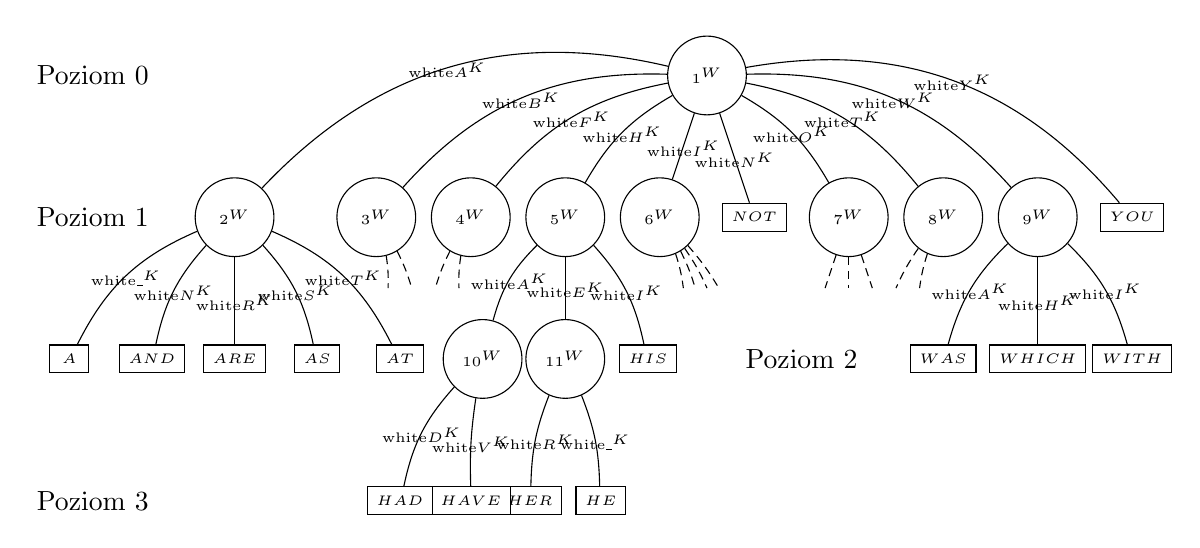
\begin{tikzpicture}[
		state/.style = { circle, top color = white, bottom color = white, draw, black, text = black, minimum width = 1 cm, font = \tiny },
		complete/.style = { rectangle, top color = white, bottom color = white, draw, black, text = black, minimum width = 0.5cm, font = \tiny}
		]
		\def\oneUnit{0.6cm}
		\def\yPosLevel{-13}
		
		\node (Level0) at (\yPosLevel*\oneUnit,0*\oneUnit) {Poziom 0};
		\node (Level1) at (\yPosLevel*\oneUnit,-3*\oneUnit) {Poziom 1};
		\node (Level2) at (2*\oneUnit,-6*\oneUnit) {Poziom 2};
		\node (Level3) at (\yPosLevel*\oneUnit,-9*\oneUnit) {Poziom 3};
		
		\node[state] (1W) at (0*\oneUnit,0*\oneUnit) {$1^W$};
		
		\node[complete] (NOT) at (1*\oneUnit,-3*\oneUnit) {\rotatedBox{$NOT$}};
		\node[state] (6W) at (-1*\oneUnit,-3*\oneUnit) {$6^W$};
		
		\node[state] (7W) at (3*\oneUnit,-3*\oneUnit) {$7^W$};
		\node[state] (5W) at (-3*\oneUnit,-3*\oneUnit) {$5^W$};
		
		\node[state] (8W) at (5*\oneUnit,-3*\oneUnit) {$8^W$};
		\node[state] (4W) at (-5*\oneUnit,-3*\oneUnit) {$4^W$};
		
		\node[state] (9W) at (7*\oneUnit,-3*\oneUnit) {$9^W$};
		\node[state] (3W) at (-7*\oneUnit,-3*\oneUnit) {$3^W$};
		
		\node[complete] (YOU) at (9*\oneUnit,-3*\oneUnit) {\rotatedBox{$YOU$}};
		\node[state] (2W) at (-10*\oneUnit,-3*\oneUnit) {$2^W$};
		
		\path (1W) edge [] node[above = -0.25 cm] {\tiny \contour{white}{$N^K$}} (NOT);
		\path (1W) edge [] node[above = -0.25 cm] {\tiny \contour{white}{$I^K$}} (6W);
		
		\path (1W) edge [bend right = -15] node[above = -0.25 cm] {\tiny \contour{white}{$O^K$}} (7W);
		\path (1W) edge [bend left = -15] node[above = -0.25 cm] {\tiny \contour{white}{$H^K$}} (5W);
		
		\path (1W) edge [bend left = -20] node[above = -0.25 cm] {\tiny \contour{white}{$F^K$}} (4W);
		\path (1W) edge [bend right = -20] node[above = -0.25 cm] {\tiny \contour{white}{$T^K$}} (8W);
		
		\path (1W) edge [bend left = -25] node[above = -0.25 cm] {\tiny \contour{white}{$B^K$}} (3W);
		\path (1W) edge [bend right = -25] node[above = -0.25 cm] {\tiny \contour{white}{$W^K$}} (9W);
		
		\path (1W) edge [bend left = -30] node[above = -0.25 cm] {\tiny \contour{white}{$A^K$}} (2W);
		\path (1W) edge [bend right = -30] node[above = -0.25 cm] {\tiny \contour{white}{$Y^K$}} (YOU);
		
		\node[complete] (WHICH) at (7*\oneUnit,-6*\oneUnit) {\rotatedBox{$WHICH$}};
		
		\node[complete] (WITH) at (9*\oneUnit,-6*\oneUnit) {\rotatedBox{$WITH$}};
		\node[complete] (WAS) at (5*\oneUnit,-6*\oneUnit) {\rotatedBox{$WAS$}};
		
		\path (9W) edge [] node[above = -0.25cm] {\tiny \contour{white}{$H^K$}} (WHICH);
		
		\path (9W) edge [bend right = -15] node[above = -0.25 cm] {\tiny \contour{white}{$I^K$}} (WITH);
		\path (9W) edge [bend left = -15] node[above = -0.25 cm] {\tiny \contour{white}{$A^K$}} (WAS);
		
		\path (8W) edge [densely dashed, bend right = 5] (4*\oneUnit,-4.5*\oneUnit);
		\path (8W) edge [densely dashed, bend right = 5] (4.5*\oneUnit,-4.5*\oneUnit);
		
		\path (7W) edge [densely dashed] (3.5*\oneUnit,-4.5*\oneUnit);
		\path (7W) edge [densely dashed] (3*\oneUnit,-4.5*\oneUnit);
		\path (7W) edge [densely dashed] (2.5*\oneUnit,-4.5*\oneUnit);
		
		\path (6W) edge [densely dashed, bend left = 5] (-0.25*\oneUnit,-4.5*\oneUnit);
		\path (6W) edge [densely dashed, bend left = 5] (-0.5*\oneUnit,-4.5*\oneUnit);
		\path (6W) edge [densely dashed, bend left = 5] (0*\oneUnit,-4.5*\oneUnit);
		\path (6W) edge [densely dashed, bend left = 5] (0.25*\oneUnit,-4.5*\oneUnit);
		
		\node[state] (11W) at (-3*\oneUnit,-6*\oneUnit) {$11^W$};
		\node[complete] (HIS) at (-1.25*\oneUnit,-6*\oneUnit) {\rotatedBox{$HIS$}};
		\node[state] (10W) at (-4.75*\oneUnit,-6*\oneUnit) {$10^W$};
		
		\path (5W) edge [] node[above = -0.25cm] {\tiny \contour{white}{$E^K$}} (11W);
		
		\path (5W) edge [bend right = -15] node[above = -0.25 cm] {\tiny \contour{white}{$I^K$}} (HIS);
		\path (5W) edge [bend left = -15] node[above = -0.25 cm] {\tiny \contour{white}{$A^K$}} (10W);
				
		\node[complete] (HE) at (-2.25*\oneUnit,-9*\oneUnit) {\rotatedBox{$HE$}};
		\node[complete] (HER) at (-3.75*\oneUnit,-9*\oneUnit) {\rotatedBox{$HER$}};
		\node[complete] (HAVE) at (-5*\oneUnit,-9*\oneUnit) {\rotatedBox{$HAVE$}};
		\node[complete] (HAD) at (-6.5*\oneUnit,-9*\oneUnit) {\rotatedBox{$HAD$}};
	
		\path (11W) edge [bend right = -10] node[above = -0.25 cm] {\tiny \contour{white}{$\_^K$}} (HE);
		\path (11W) edge [bend left = -10] node[above = -0.25 cm] {\tiny \contour{white}{$R^K$}} (HER);
		
		\path (10W) edge [bend left = -5] node[above = -0.25 cm] {\tiny \contour{white}{$V^K$}} (HAVE);
		\path (10W) edge [bend left = -15] node[above = -0.25 cm] {\tiny \contour{white}{$D^K$}} (HAD);
		
		\path (4W) edge [densely dashed, bend right = 5] (-5.25*\oneUnit,-4.5*\oneUnit);
		\path (4W) edge [densely dashed, bend right = 5] (-5.75*\oneUnit,-4.5*\oneUnit);
		
		\path (3W) edge [densely dashed, bend left = 5] (-6.75*\oneUnit,-4.5*\oneUnit);
		\path (3W) edge [densely dashed, bend left = 5] (-6.25*\oneUnit,-4.5*\oneUnit);
		
		\node[complete] (ARE) at (-10*\oneUnit,-6*\oneUnit) {\rotatedBox{$ARE$}};
		
		\node[complete] (AS) at (-8.25*\oneUnit,-6*\oneUnit) {\rotatedBox{$AS$}};
		\node[complete] (AND) at (-11.75*\oneUnit,-6*\oneUnit) {\rotatedBox{$AND$}};
		
		
		\node[complete] (AT) at (-6.5*\oneUnit,-6*\oneUnit) {\rotatedBox{$AT$}};
		\node[complete] (A) at (-13.5*\oneUnit,-6*\oneUnit) {\rotatedBox{$A$}};
		
		\path (2W) edge [] node[above = -0.25cm] {\tiny \contour{white}{$R^K$}} (ARE);
		
		\path (2W) edge [bend right = -15] node[above = -0.25 cm] {\tiny \contour{white}{$S^K$}} (AS);
		\path (2W) edge [bend left = -15] node[above = -0.25 cm] {\tiny \contour{white}{$N^K$}} (AND);
		
		\path (2W) edge [bend right = -20] node[above = -0.25 cm] {\tiny \contour{white}{$T^K$}} (AT);
		\path (2W) edge [bend left = -20] node[above = -0.25 cm] {\tiny \contour{white}{$\_^K$}} (A);
		\end{tikzpicture}
			
		\begin{tablenotes}
			\centering
			\footnotesize
			\item $n^W$ -- Identyfikator (numer) węzła.
			\item $n^K$ -- Identyfikator gałęzi (znak pozwalający na przejście z jednego węzła do drugiego).
			\item $\_^K$ -- Znak o wartości pustej, braku znaku.
		\end{tablenotes}
	\end{figure}
	
	Warto również zwrócić uwagę na schemat drzewa~\ref{fig:CompleteTrieTree} ze względu na unikalną gałąź $\_^K$ z węzła $2^W$ do węzła $A$ w przypadku naszej struktury \emph{Trie}. Prefiksem węzła $2^W$ jest litera \texttt{A}.
	
	\ifsourcematerial
	\begin{displayquote}
		\color{ao(english)}
		\underline{\textbf{FRAGMENT TŁUMACZONY:}} \newline
		\elide If we pursue the thumb-index idea to one of its logical conclusions, we come
		up with a searching scheme based on repeated “subscripting” as illustrated in
		Table 1. Suppose that we want to test a given search argument to see whether it
		is one of the 31 most common words of English (see Figs. 12 and 13 in Section
		6.2.2). \elide 
		
		\textbf{\color{ao(english)} Example}
		
		For example, the trie of Table 1 has 12 nodes; node (1) is the root, and we
		look up the first letter here. If the first letter is, say, \emph{N}, the table tells us that our word must be \emph{NOT} (or else it isn’t in the table). On the other hand, if the first letter is \emph{W}, node (1) tells us to go on to node (9), looking up the second letter in the same way; node (9) says that the second letter should be \emph{A}, \emph{H}, or \emph{I}. The prefix of node (10) is \emph{HA}. Blank entries in the table stand for null links.
	\end{displayquote}
	\fi
	
	Knuth podkreśla w swojej książce~\cite{KnuthsTheArtOfComputerProgramming3}, że wektory węzłów w tablicy~\ref{tab:trieTreeFor31MostCommonEnglishWords} są ułożone w~kolejności odpowiadającej kolejności ułożenia znaków w maszynie \emph{MIX}. Miało to szczególne znaczenie w momencie, kiedy pisał on swoją książkę, gdyż język \emph{MIX} przypominał kod maszynowy komputerów w czasie jego opracowania -- przed 1969 rokiem.
	
    Wszystko to miało wpływ na zwiększenie prędkości przeszukiwania drzewa \emph{Trie}, ponieważ postępując zgodnie z algorytmem Knuth'a jedynie wyciągamy słowa z tablicy, używając znaków naszych kluczy jako indeksów, a nie przeszukujemy wektory, aby znaleźć odpowiednią w niej wartość. Aspektem, który stara się tutaj podkreślić Knuth jest różnica pomiędzy przeszukiwaniem tablicy (ang. \emph{table look-up}), a ''zaglądaniem do tablicy'' (ang. \emph{table look-at}) w ściśle określone miejsce.
	
	\ifsourcematerial
	\begin{displayquote}
		\color{ao(english)}
		\underline{\textbf{FRAGMENT TŁUMACZONY:}} \newline
		The node vectors in Table 1 are arranged according to \emph{MIX} character code. 
		
		[MIX is decidedly not an esoteric language, it deliberately resembles the languages of real computers at the time it was invented (before 1969).] 
		
		This means that a trie search will be quite fast, since we are merely fetching words of an array by using the characters of our keys as subscripts. Techniques
		for making quick multiway decisions by subscripting have been called “table
		look-at” as opposed to “table look-up” [see P. M. Sherman, CACM 4 (1961),
		172–173, 175].
	\end{displayquote}
	\fi
	
	\subsubsection{Algorytm T -- Przeszukiwanie \emph{Trie}}\label{sec:AlgorytmT}
	
	Inaczej określane w polskiej wersji książki Knuth'a jako ,,wyszukiwanie w drzewie \emph{Trie}`` -- algorytm wyszukuje argument $K$ w posiadanej tablicy.
	
	\textbf{Założenia}: 
	
    Dana jest tablica wektorów o $M$ elementach, tworzącą \emph{M-ary} drzewo. Indeksy wektorów zaczynają się od $0$, a kończą na $M-1$. Elementem tych wektorów może być klucz -- całe słowo znajdujące się w tablicy -- lub odniesienia do następnego wektora. Jeżeli element takiego wektora jest pusty, równy \emph{null}, oznacza to, że słowo, które obecnie próbujemy dopasować nie istnieje wewnątrz naszej struktury \emph{Trie}. Jeżeli jednak znajdziemy całe słowo -- klucz -- i jest ono takie samo jako ciąg znaków, który próbujemy dopasować. Oznacza to, że argument przeszukiwania $K$ należy do naszego drzewa \emph{Trie}.
		
	\begin{enumerate}
		\item \textbf{Inicjalizacja} \newline
		Ustaw $P$ -- odniesienie do obecnego wektora -- tak, aby wskazywało na korzeń drzewa.
		\item \textbf{Rozgałęzienie} \newline
		Ustaw $k$ -- kod naszego obecnie przetwarzanego znaku z argumentu wejściowego $K$ -- na kod znaku następnego w kolejności od lewej do prawej. \newline
		Jeżeli argument wejściowy $K$ został przetworzony w całości należy ustawić $k$ na znak pusty lub znak odpowiadający końcowi słowa. \newline
		Reprezentacja znaku powinna przyjmować wartość w zakresie $0\leq k < M$. Jest to liczba całkowita oznaczająca kod znaku. \newline
		$X$ jest wartością komórki o indeksie $k$ wektora $P$. $P(k) = X$
		\begin{enumerate}
			\item Jeżeli $X$ jest odniesieniem do kolejnego wektora -- idź do punktu 3.
			\item Jeżeli $X$ jest kluczem -- idź do punktu 4.
		\end{enumerate}
		\item \textbf{Postęp} 
		\begin{enumerate} 
			\item Jeżeli $X$ jest odniesieniem do jednego z wektorów, nie jest pustym, \emph{null} wskaźnikiem -- podstaw $X$ pod $P$ i idź do punktu 2.
			\item Jeżeli $X$ nie jest odniesieniem do jednego z wektorów -- zakończ z niepowodzeniem.
		\end{enumerate}
		\item \textbf{Porównanie} 
		\begin{enumerate}
			\item Jeżeli $X$ = $K$, jest całym argumentem wejściowym -- zakończ z powodzeniem.
			\item Jeżeli $X$ $\neq$ $K$ -- zakończ z niepowodzeniem. \newline
		\end{enumerate}			
	\end{enumerate}
	
	Dodatkowo należy zwrócić uwagę na fakt, że jeżeli nie znajdziemy słowa w naszej strukturze to znajdujemy najdłuższy fragment pasujący -- najdłuższe dopasowanie.
	
	\ifsourcematerial
	\begin{displayquote}
		\color{ao(english)}
		\underline{\textbf{FRAGMENT TŁUMACZONY:}} \newline
		Algorithm T (Trie search). Given a table of records that form an M-ary trie, this
		algorithm searches for a given argument K. The nodes of the trie are vectors
		whose subscripts run from 0 to M - 1; each component of these vectors is either
		a key or a link (possibly null). \newline
		T1. [Initialize.] Set the link variable so that it points to the root of the trie. \newline
		T2. [Branch.] Set k to the next character of the input argument, K, from left
		to right. (If the argument has been completely scanned, we set k to a
		“blank” or end-of-word symbol. The character should be represented as
		a number in the range 0 <= k < M.) Let X be table entry number k in
		. If X is a link, go to T3; but if X is a key, go to T4. \newline
		T3. [Advance.] If X = $\Lambda$ [$\Lambda$ - null pointer], set P <- X and return to step T2; otherwise the
		algorithm terminates unsuccessfully. \newline
		T4. [Compare.] If X = K, the algorithm terminates successfully; otherwise it
		terminates unsuccessfully. 
		
		Notice that if the search is unsuccessful, the longest match has been found.
		This property is occasionally useful in applications.
	\end{displayquote}
	\fi
	
	\subsubsection{Przeznaczenie}\label{sec:AlgorytmTPrzeznaczenie}
	
	Knuth w celu porównania omawianych algorytmów tworzy krótki program na maszynę \emph{MIX}, który jest implementacją algorytmu T~\ref{sec:AlgorytmT}. Dzięki wykorzystaniu maszyny \emph{MIX} może on przyjąć wiele założeń, które mogą znacząco wpłynąć na wyniki testów wydajnościowych. 
	
	Przede wszystkim Knuth zakłada, że pojedyncze znaki mają długość jednego bajtu, a klucze mają co najwyżej długość 5 bajtów. Niestety posługując się językiem \emph{Java} -- gdzie na \emph{char} czy pojedynczy znak w \emph{Stringu} do przetrzymywania w pamięci potrzebne są 2 bajty -- jesteśmy z góry ograniczeni założeniami języka.
	
    Dodatkowo Knuth przyjmuje, że każdy z kluczy reprezentowany jest jako jedno słowo -- o długości 5 znaków -- zakodowane przez maszynę \emph{MIX}, gdzie puste, niewypełnione przez klucz miejsca zastąpione są przez znak odstępu -- spację. Puste miejsca znajdują się po prawej stronie, a klucz zaczynamy wpisywać od lewej strony słowa.
	
    Ułatwieniem również jest kodowanie znaków \emph{MIX} z czym wiąże się reprezentacja każdego z bajtów argumentu przeszukiwania $K$ w postaci numeru mniejszego od 30. Ponownie \emph{Java} różni się tutaj reprezentacją w kodzie znaków w standardzie UTF-16. Szczególnym problemem jest tutaj sposób dowiązań przyjęty przez Knuth'a, który reprezentowany jest poprzez liczby ujemne w zbiorze \{0,1,2\} słowa odpowiadającego węzłowi.
	
	\subsubsection{Złożoność czasowa i pamięciowa}\label{sec:AlgorytmTZlozonoscCzasowaIPamieciowa}
	
    Najważniejsze tutaj są jednak wnioski, do jakich doszedł Knuth. Wykonywanie jego programu zajmuje $8*C+8$ jednostek czasu, gdzie $C$ jest ilością znaków przetworzonych. Jako że $C\leq5$ to przeszukiwanie nigdy nie zajmie dłużej niż 48 jednostek czasu.
    
	Struktura \emph{Trie} zajmuje natomiast znacznie więcej pamięci. Używamy 360 słów do reprezentacji 31 kluczy. Dla porównania, w przypadku gdy kontenerem przechowującym dane byłoby drzewo binarne, użylibyśmy 62 słów.
	
	Na szczęście Knuth przedstawił pomysł na rozwiązanie tego problemu w postaci reorganizacji struktury tablicowej do skompresowanej tablicy dwuwymiarowej.
	
	Porównując Algorytm T~\ref{sec:AlgorytmT} do programu optymalnego przeszukiwania binarnego drzewa dla tego samego zbioru argumentów przeszukiwania $K$ -- Knuth zauważa, że:
	
	\begin{itemize}
		\item Program implementujący algorytm T oraz optymalne przeszukiwanie binarnego drzewa w przypadku sukcesu zajmują 26 jednostek czasu.
		\item Przeszukiwanie \emph{Trie} jest zdecydowanie szybsze w przypadkach kończących się niepowodzeniem. Dodatkowo w sytuacji, w której użyjemy omawianych danych, dużo częściej będziemy mieć do czynienia z nieznalezieniem poszukiwanego słowa w naszym zbiorze.
		\item Knuth dodatkowo nawiązuje do odmiennego podejścia do problemu w postaci indeksowania KWIC (ang. \emph{keyword in context})%
		\footnote{Wykorzystanie w kontekście optymalnego przeszukiwania binarnego w \emph{Sztuce Programowania} na stronach 560 - 561~\cite{KnuthsTheArtOfComputerProgramming3}. Pomysł KWIC zaproponowany w 
			H. P. Luhn, Amer. Documentation 11 (1960), 288–295. Pełne indeksowanie KWIC znajduje się w W. W. Youden, JACM 10 (1963), 583–646. 
		}.
		Zauważa on, że w tym przypadku zastosowanie \emph{Trie} nie ma sensu w klasycznym znaczeniu z powodu natury danych zawartych w strukturze. Ponownie przedstawia nietuzinkowe rozwiązaniem jakim jest przetwarzanie słów od prawej strony do lewej, tak aby odróżnienie słów takich jak \texttt{COMPUTATION} i \texttt{COMPUTATIONS} nie zajmowało 12 iteracji.
	\end{itemize}
	
	\ifsourcematerial
	\begin{displayquote}
		\color{ao(english)}
		\underline{\textbf{FRAGMENT TŁUMACZONY:}} \newline
		In order to compare the speed of this algorithm to the others in this chapter, we can write a short program assuming that the characters are bytes and that the keys are at most five bytes long. \newline
		
		\textbf{Program T} (\emph{Trie} search). This program assumes that all keys are represented in one \texttt{MIX} word, with blank spaces at the right whenever the key has less than five characters. Since we use \texttt{MIX} character code, each byte of the search argument is assumed to contain a number less than 30. Links are represented as negative numbers in the 0:2 field of a node word. rI1 = \texttt{P}, rX = unscanned part of \texttt{K}.
		
		\elide Treść programu w języku MIX. \elide
		
		The running time of this program is 8C + 8 units, where C is the number of
		characters examined. Since C <= 5, the search never needs more than 48 units of 
		time.
		
		If we now compare the efficiency of this program (using the trie of Table 1)
		to Program 6.2.2T (using the optimum binary search tree of Fig. 13), we can
		make the following observations.
		
		1. The trie takes much more memory space; we are using 360 words just to
		represent 31 keys, while the binary search tree uses only 62 words of memory.
		(However, exercise 4 shows that, with some fiddling around, we can actually fit
		the trie of Table 1 into only 49 words.)
		
		2. A successful search takes about 26 units of time for both programs. But an
		unsuccessful search will go faster in the trie, slower in the binary search tree. For
		this data the search will be unsuccessful more often than it is successful, so the
		trie is preferable from the standpoint of speed.
		
		3. If we consider the KWIC indexing application of Fig. 15 instead of the 31
		commonest English words, the trie loses its advantage because of the nature of
		the data. For example, a trie requires 12 iterations to distinguish between \texttt{COMPUTATION} and \texttt{COMPUTATIONS}. In this case it would be better to build the trie so that words are scanned from right to left instead of from left to right.
	\end{displayquote}
	\fi
	
	\subsubsection{Drzewo \emph{Trie} reprezentowane przez skompresowaną tablicę dwuwymiarową}\label{sec:DrzwoTrieReprezentowanePrzezSkommpresowanaTabliceDwuwymiarowa}
	
	Skompresowana tablica dwuwymiarowa powstaje przez nakładanie komórek zajętych na te, które są puste. W ten sposób otrzymujemy tablicę postaci przedstawionej w poniższej tablicy~\ref{tab:compressedTrieTreeFor31MostCommonEnglishWords}.
	
    Do skompresowanej w ten sposób tablicy potrzebny jest oddzielny algorytm przeszukiwania. Knuth opisuje ten algorytm w jednym z wcześniejszych rozdziałów w postaci programu napisanego dla maszyny \emph{MIX} (,,Program T`` w rozdziale 6.2.2. ,,Wyszukiwanie w drzewach binarnych`` - ang. \emph{,,Binary Tree Searching``}~\cite{KnuthsTheArtOfComputerProgramming3}). Nie będzie on jednak działa tak szybko, jak algorytm dla nieskompresowanej tablicy. Należy jednak wziąć pod uwagę fakt, że większa część z 360 komórek w tablicy~\ref{tab:trieTreeFor31MostCommonEnglishWords} jest pusta, a przekształcając tablicę do formy skompresowanej, zmniejszamy ilość wszystkich komórek do 49.
    
	\ifsourcematerial
	\begin{displayquote}
		\color{ao(english)}
		\underline{\textbf{FRAGMENT TŁUMACZONY:}} \newline
		
		The trie takes much more memory space; we are using 360 words just to
		represent 31 keys, while the binary search tree uses only 62 words of memory.
		(However, exercise 4 shows that, with some fiddling around, we can actually fit
		the trie of Table 1 into only 49 words.
		
		\textbf{Exercise 4}. [21] Most of the 360 entries in Table 1 are blank (null links). But we can
		compress the table into only 49 entries, by overlapping nonblank entries with
		blank ones as follows:
		
		(Nodes (1), (2), . . ., (12) of Table 1 begin, respectively, at positions 20, 19, 3, 14,
		1, 17, 1, 7, 3, 20, 18, 4 within this compressed table.)
		Show that if the compressed table is substituted for Table 1, Program T will
		still work, but not quite as fast.
	\end{displayquote}
	\fi
	\begin{table}
		\centering
		\begin{threeparttable}
			\caption{Schemat skompresowanej tablicy dwuwymiarowej reprezentującej drzewo \emph{Trie} dla 31 najpopularniejszych słów angielskich. Tablica powstała na podstawie tablicy~\ref{tab:trieTreeFor31MostCommonEnglishWords} poprzez nałożenie komórek zajętych na te, które są puste. Identyfikatory węzłów w tej tabeli (pojawiające się w~wierszach ,,Start węzła`` bądź ,,Zawartość``) odpowiadają identyfikatorom z tabeli~\ref{tab:trieTreeFor31MostCommonEnglishWords}. W wierszach ,,Zawartość`` oprócz identyfikatorów węzłów można znaleźć klucze (pełne słowa). Tablica jest zasięgnięta z książki Knuth'a~\cite{KnuthsTheArtOfComputerProgramming3}.}\label{tab:compressedTrieTreeFor31MostCommonEnglishWords}
			
			{ \small
				\begin{tabularx}{\textwidth}{C{5.4}|C{1.2}|C{1.2}|C{1.2}|C{1.2}|C{1.2}|C{1.2}|C{1.2}|C{1.2}|C{1.2}|C{1.2}|C{1.2}|C{1.2}|C{1.2}|C{1.2}}
					Pozycja & 1 & 2 & 3 & 4 & 5 & 6 & 7 & 8 & 9 & 10 & 11 & 12 & 13 & 14 \\
					\toprule
					Start & 5\tnote{W} && 3\tnote{W} &&&&&&&&&&& \\
					węzła & 7\tnote{W} && 9\tnote{W} & 12\tnote{W} &&& 8\tnote{W} &&&&&&& 4\tnote{W} \\
					\hline
					Zawartość &&&& \texttt{W} & \texttt{T} && \texttt{O} & \texttt{B} & \texttt{T} & \texttt{H} & \texttt{W} & \texttt{W} & \texttt{T} & \\
					
					&& \texttt{10\tnote{W}} && \texttt{A} & \texttt{H} & \texttt{11\tnote{W}} & \texttt{F} & \texttt{E} & \texttt{H} & \texttt{I} & \texttt{H} & \texttt{I} & \texttt{H} & \\
					
					&&&& \texttt{S} & \texttt{A} &&&& \texttt{E} & \texttt{S} & \texttt{I} & \texttt{T} & \texttt{I} & \\
					
					&&&&            & \texttt{T} &&&&&& \texttt{C} & \texttt{H} & \texttt{S} & \\
					
					&&&&&&&&&&& \texttt{H} &&& \\
					\hline
					\hline
				\end{tabularx}
			}
			
			
			%			1 <- $5^W$, $7^W$ \\
			%			3 <- $3^W$, $9^W$ \\
			%			4 <- $12^W$ \\
			%			7 <- $8^W$ \\
			%			14 <- $4^W$ \\
			%			---------------------- \\
			%			17 <- $6^W$ \\
			%			18 <- $11^W$ \\
			%			19 <- $2^W$ \\
			%			20 <- $1^W$, $10^W$ \\
			
			{ \small
				\begin{tabularx}{\textwidth}{C{5.4}|C{1.2}|C{1.2}|C{1.2}|C{1.2}|C{1.2}|C{1.2}|C{1.2}|C{1.2}|C{1.2}|C{1.2}|C{1.2}|C{1.2}|C{1.2}|C{1.2}}
					Pozycja & 15 & 16 & 17 & 18 & 19 & 20 & 21 & 22 & 23 & 24 & 25 & 26 & 27 & 28 \\
					\toprule 
					Start & &&&&& 1\tnote{W} &&&&&&&& \\
					węzła & && 6\tnote{W} & 11\tnote{W} & 2\tnote{W} & 10\tnote{W} &&&&&&&& \\
					\hline
					Zawartość && \texttt{O} & \texttt{I} & \texttt{H} & \texttt{A} & \texttt{O} &&& \texttt{T} & \texttt{H} &&& \texttt{B} & \\
					
					& \texttt{12\tnote{W}} & \texttt{N} && \texttt{E} && \texttt{R} & \texttt{2\tnote{W}} & \texttt{3\tnote{W}} & \texttt{O} & \texttt{A} && \texttt{4\tnote{W}} & \texttt{U} & \texttt{5\tnote{W}} \\
					
					&&&&&&&&&& \texttt{D} &&& \texttt{T} & \\
					\hline
					\hline
				\end{tabularx}
			}
			
			{ \small
				\begin{tabularx}{\textwidth}{C{5.4}|C{1.2}|C{1.2}|C{1.2}|C{1.2}|C{1.2}|C{1.2}|C{1.2}|C{1.2}|C{1.2}|C{1.2}|C{1.2}|C{1.2}|C{1.2}|C{1.2}}
					Pozycja & 29 & 30 & 31 & 32 & 33 & 34 & 35 & 36 & 37 & 38 & 39 & 40 & 41 & 42 \\
					\toprule 
					Zawartość & & \texttt{F} & \texttt{B} & \texttt{I} & \texttt{F} & \texttt{A} & \texttt{N} & & \texttt{H} & \texttt{A} & \texttt{I} & \texttt{I} & \texttt{A} & \texttt{A} \\
					
					& \texttt{6\tnote{W}} & \texttt{O} & \texttt{Y} & \texttt{N} & \texttt{R} & \texttt{N} & \texttt{O} & \texttt{7\tnote{W}} & \texttt{E} & \texttt{R} & \texttt{S} & \texttt{T} & \texttt{S} & \texttt{T} \\
					
					& & \texttt{R} &&& \texttt{O} & \texttt{D} & \texttt{T} & &  \texttt{R} & \texttt{E} &&&& \\
					&&&&& \texttt{M} &&&&&&&&& \\
					\hline
					\hline
				\end{tabularx}
			}
			
			{ \small
				\begin{tabularx}{0.575\textwidth}{C{5.4}|C{1.2}|C{1.2}|C{1.2}|C{1.2}|C{1.2}|C{1.2}|C{1.2}}
					Pozycja & 43 & 44 & 45 & 46 & 47 & 48 & 49 \\
					\toprule 
					Zawartość & & & \texttt{H} & & & \texttt{Y} & \\
					
					& \texttt{8\tnote{W}} & & \texttt{A} & \texttt{9\tnote{W}} & & \texttt{O} & \\
					
					& & & \texttt{V} & & & \texttt{U} & \\
					& & & \texttt{E} & & & & \\
					\hline
				\end{tabularx}
			}
			
			%				\begin{tablenotes}
			%					\centering
			%					\footnotesize
			%					\item[W] - Numer węzła
			%				\end{tablenotes}
		\end{threeparttable}
	\end{table}
	
	\ifsourcematerial
	\begin{displayquote}
		\color{ao(english)}
		\underline{\textbf{FRAGMENT TŁUMACZONY:}} \newline
		
		\textbf{Exercise 4}. Solution. Successful searches take place exactly as with the full table, but
		unsuccessful searches in the compressed table may go through several
		additional iterations. For example, an input argument such as \texttt{TRASH} will
		make Program T take six iterations (more than five!); this is the worst case. It
		is necessary to verify that no infinite looping on blank sequences is possible.
		(This remarkable 49-place packing is due to J. Scot Fishburn, who also showed
		that 48 places do not suffice.)
		
		A slower but more versatile way to economize on trie storage has beenproposed by Kurt Maly, CACM 19 (1976), 409–415.
		
		In general, if we want to compress n sparse tables containing respectively
		x 1 , . . ., x n nonzero entries, a first-fit method that offsets the jth table by the
		minimum amount r j that will not conflict with the previously placed tables
		will have r j =< (x 1 + ... + x j-1 )x j , since each previous nonzero entry can block
		at most x j offsets. This worst-case estimate gives r j <= 93 for the data in Table
		1, guaranteeing that any twelve tables of length 30 containing respectively 10,
		5, 4, 3, 3, 3, 3, 3, 2, 2, 2, 2 nonzero entries can be packed into 93 + 30
		consecutive locations regardless of the pattern of the nonzeros. Further
		refinements of this method have been developed by R. E. Tarjan and A. C.
		Yao, CACM 22 (1979), 606–611. A dynamic implementation of compressed
		tries, due to F. M. Liang, is used for hyphenation tables in the TeX typesetting
		system. [See D. E. Knuth, CACM 29 (1986), 471–478; Literate Programming
		(1992), 206–233.]
	\end{displayquote}
	\fi
	
	\subsection{Las \emph{Trie}}\label{sec:LasTrie}
	Kolejną strukturą na której Knuth buduje swoje rozważania jest las zaproponowany przez René de la Briandais~\cite{BriandaisWesternJointComputerConf}. Modyfikacja konstrukcji drzewa \emph{Trie}, przedstawiona przez René, polega na zamianie każdego węzła z postaci wektora na \emph{linked} listę. Zaletą tego rozwiązania jest eliminacja węzłów pustych z drzewa, co można zobaczyć na rysunku~\ref{fig:CompleteTrieForest} przedstawiającym graficzną reprezentację schemat lasu \emph{Trie}.
	
	\begin{figure}[H]
		\caption{Graficzna reprezentacja schematu lasu drzew \emph{Trie} dla 21 wybranych słów ze zbioru 31 słów najczęściej występujących w języku angielskim. Węzły zawierające litery \texttt{H}, \texttt{I}, \texttt{N}, \texttt{O}, \texttt{T}, \texttt{W}, \texttt{Y} są korzeniami drzew, zawierających słowa, dla których znak z korzenia jest prefiksem. Znak końca wspólny dla wszystkich drzew, jest unikalnym, wcześniej ustalonym znakiem i pojawia się na końcu każdego klucza. Figura zasięgnięta jest z książki Knuth'a~\cite{KnuthsTheArtOfComputerProgramming3}.}\label{fig:CompleteTrieForest}
		\centering 
		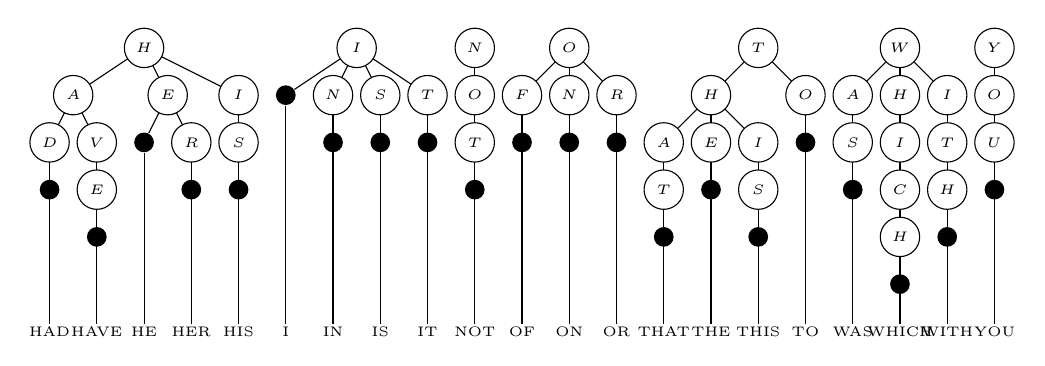
\begin{tikzpicture}[
		state/.style = { circle, top color = white, bottom color = white, draw, black, text = black, minimum width = 0.5 cm, font = \tiny, inner sep=0pt, outer sep=0pt },
		comp/.style = {font = \tiny, inner sep=0.5pt, outer sep=0.5pt},
		end/.style = { circle, fill, color = black, inner sep=0pt, minimum width = 0.25 cm }
		]
		\def\oneUnit{0.6cm}
		
		\node[state] (H) at (-9*\oneUnit,5*\oneUnit) {$H$};
		\node[state] (I) at (-4.5*\oneUnit,5*\oneUnit) {$I$};
		\node[state] (N) at (-2*\oneUnit,5*\oneUnit) {$N$};
		\node[state] (O) at (0*\oneUnit,5*\oneUnit) {$O$};
		\node[state] (T) at (4*\oneUnit,5*\oneUnit) {$T$};
		\node[state] (W) at (7*\oneUnit,5*\oneUnit) {$W$};
		\node[state] (Y) at (9*\oneUnit,5*\oneUnit) {$Y$};
		
		\node[state] (A21) at (-10.5*\oneUnit,4*\oneUnit) {$A$};
		\node[state] (E2) at (-8.5*\oneUnit,4*\oneUnit) {$E$};
		\node[state] (I21) at (-7*\oneUnit,4*\oneUnit) {$I$};
		\node[end] (IEnd) at (-6*\oneUnit,4*\oneUnit) {};
		\node[state] (N21) at (-5*\oneUnit,4*\oneUnit) {$N$};
		\node[state] (S2) at (-4*\oneUnit,4*\oneUnit) {$S$};
		\node[state] (T2) at (-3*\oneUnit,4*\oneUnit) {$T$};
		\node[state] (O21) at (-2*\oneUnit,4*\oneUnit) {$O$};
		\node[state] (F2) at (-1*\oneUnit,4*\oneUnit) {$F$};
		\node[state] (N22) at (0*\oneUnit,4*\oneUnit) {$N$};
		\node[state] (R2) at (1*\oneUnit,4*\oneUnit) {$R$};
		\node[state] (H21) at (3*\oneUnit,4*\oneUnit) {$H$};
		\node[state] (O22) at (5*\oneUnit,4*\oneUnit) {$O$};
		\node[state] (A22) at (6*\oneUnit,4*\oneUnit) {$A$};
		\node[state] (H22) at (7*\oneUnit,4*\oneUnit) {$H$};
		\node[state] (I22) at (8*\oneUnit,4*\oneUnit) {$I$};
		\node[state] (O23) at (9*\oneUnit,4*\oneUnit) {$O$};
		
		\node[state] (D3) at (-11*\oneUnit,3*\oneUnit) {$D$};
		\node[state] (V3) at (-10*\oneUnit,3*\oneUnit) {$V$};
		\node[end] (HeEnd) at (-9*\oneUnit,3*\oneUnit) {};
		\node[state] (R3) at (-8*\oneUnit,3*\oneUnit) {$R$};
		\node[state] (S31) at (-7*\oneUnit,3*\oneUnit) {$S$};
		\node[end] (InEnd) at (-5*\oneUnit,3*\oneUnit) {};
		\node[end] (IsEnd) at (-4*\oneUnit,3*\oneUnit) {};
		\node[end] (ItEnd) at (-3*\oneUnit,3*\oneUnit) {};
		\node[state] (T31) at (-2*\oneUnit,3*\oneUnit) {$T$};
		\node[end] (OfEnd) at (-1*\oneUnit,3*\oneUnit) {};
		\node[end] (OnEnd) at (0*\oneUnit,3*\oneUnit) {};
		\node[state] (A3) at (2*\oneUnit,3*\oneUnit) {$A$};
		\node[end] (OrEnd) at (1*\oneUnit,3*\oneUnit) {};
		\node[state] (E3) at (3*\oneUnit,3*\oneUnit) {$E$};
		\node[state] (I31) at (4*\oneUnit,3*\oneUnit) {$I$};
		\node[end] (ToEnd) at (5*\oneUnit,3*\oneUnit) {};
		\node[state] (S32) at (6*\oneUnit,3*\oneUnit) {$S$};
		\node[state] (I32) at (7*\oneUnit,3*\oneUnit) {$I$};
		\node[state] (T32) at (8*\oneUnit,3*\oneUnit) {$T$};
		\node[state] (U3) at (9*\oneUnit,3*\oneUnit) {$U$};
		
		\node[end] (HadEnd) at (-11*\oneUnit,2*\oneUnit) {};
		\node[state] (E4) at (-10*\oneUnit,2*\oneUnit) {$E$};
		\node[end] (HerEnd) at (-8*\oneUnit,2*\oneUnit) {};
		\node[end] (HisEnd) at (-7*\oneUnit,2*\oneUnit) {};
		\node[end] (NotEnd) at (-2*\oneUnit,2*\oneUnit) {};
		\node[state] (T4) at (2*\oneUnit,2*\oneUnit) {$T$};
		\node[end] (TheEnd) at (3*\oneUnit,2*\oneUnit) {};
		\node[state] (S4) at (4*\oneUnit,2*\oneUnit) {$S$};
		\node[end] (WasEnd) at (6*\oneUnit,2*\oneUnit) {};
		\node[state] (C4) at (7*\oneUnit,2*\oneUnit) {$C$};
		\node[state] (H4) at (8*\oneUnit,2*\oneUnit) {$H$};
		\node[end] (YouEnd) at (9*\oneUnit,2*\oneUnit) {};
		
		\node[end] (HaveEnd) at (-10*\oneUnit,1*\oneUnit) {};
		\node[end] (ThatEnd) at (2*\oneUnit,1*\oneUnit) {};
		\node[end] (ThisEnd) at (4*\oneUnit,1*\oneUnit) {};
		\node[state] (H5) at (7*\oneUnit,1*\oneUnit) {$H$};
		\node[end] (WithEnd) at (8*\oneUnit,1*\oneUnit) {};
		
		\node[end] (WhichEnd) at (7*\oneUnit,0*\oneUnit) {};
		
		\node[comp] (compHAD) at (-11*\oneUnit,-1*\oneUnit) {\rotatedBox{HAD}};
		\node[comp] (compHAVE) at (-10*\oneUnit,-1*\oneUnit) {\rotatedBox{HAVE}};
		\node[comp] (compHE) at (-9*\oneUnit,-1*\oneUnit) {\rotatedBox{HE}};
		\node[comp] (compHER) at (-8*\oneUnit,-1*\oneUnit) {\rotatedBox{HER}};
		\node[comp] (compHIS) at (-7*\oneUnit,-1*\oneUnit) {\rotatedBox{HIS}};
		\node[comp] (compI) at (-6*\oneUnit,-1*\oneUnit) {\rotatedBox{I}};
		\node[comp] (compIN) at (-5*\oneUnit,-1*\oneUnit) {\rotatedBox{IN}};
		\node[comp] (compIS) at (-4*\oneUnit,-1*\oneUnit) {\rotatedBox{IS}};
		\node[comp] (compIT) at (-3*\oneUnit,-1*\oneUnit) {\rotatedBox{IT}};
		\node[comp] (compNOT) at (-2*\oneUnit,-1*\oneUnit) {\rotatedBox{NOT}};
		\node[comp] (compOF) at (-1*\oneUnit,-1*\oneUnit) {\rotatedBox{OF}};
		\node[comp] (compON) at (0*\oneUnit,-1*\oneUnit) {\rotatedBox{ON}};
		\node[comp] (compOR) at (1*\oneUnit,-1*\oneUnit) {\rotatedBox{OR}};
		\node[comp] (compTHAT) at (2*\oneUnit,-1*\oneUnit) {\rotatedBox{THAT}};
		\node[comp] (compTHE) at (3*\oneUnit,-1*\oneUnit) {\rotatedBox{THE}};
		\node[comp] (compTHIS) at (4*\oneUnit,-1*\oneUnit) {\rotatedBox{THIS}};
		\node[comp] (compTO) at (5*\oneUnit,-1*\oneUnit) {\rotatedBox{TO}};
		\node[comp] (compWAS) at (6*\oneUnit,-1*\oneUnit) {\rotatedBox{WAS}};
		\node[comp] (compWHICH) at (7*\oneUnit,-1*\oneUnit) {\rotatedBox{WHICH}};
		\node[comp] (compWITH) at (8*\oneUnit,-1*\oneUnit) {\rotatedBox{WITH}};
		\node[comp] (compYOU) at (9*\oneUnit,-1*\oneUnit) {\rotatedBox{YOU}};
		
		\path (H) edge [] (A21);
		\path (H) edge [] (E2);
		\path (H) edge [] (I21);
		\path (I) edge [] (IEnd);
		\path (I) edge [] (N21);
		\path (I) edge [] (S2);
		\path (I) edge [] (T2);
		\path (N) edge [] (O21);
		\path (O) edge [] (F2);
		\path (O) edge [] (N22);
		\path (O) edge [] (R2);
		\path (T) edge [] (H21);
		\path (T) edge [] (O22);
		\path (W) edge [] (A22);
		\path (W) edge [] (H22);
		\path (W) edge [] (I22);
		\path (Y) edge [] (O23);
		
		
		\path (A21) edge [] (D3);
		\path (A21) edge [] (V3);
		\path (E2) edge [] (HeEnd);
		\path (E2) edge [] (R3);
		\path (I21) edge [] (S31);
		\path (IEnd) edge [] (compI);
		\path (N21) edge [] (compIN);
		\path (S2) edge [] (compIS);
		\path (T2) edge [] (compIT);
		\path (F2) edge [] (compOF);
		\path (N22) edge [] (compON);
		\path (R2) edge [] (compOR);
		\path (O21) edge [] (T31);
		\path (H21) edge [] (A3);
		\path (H21) edge [] (E3);
		\path (H21) edge [] (I31);
		\path (O22) edge [] (compTO);
		\path (A22) edge [] (S32);
		\path (H22) edge [] (I32);
		\path (I22) edge [] (T32);
		\path (O23) edge [] (U3);
		
		\path (D3) edge [] (compHAD);
		\path (V3) edge [] (E4);
		\path (HeEnd) edge [] (compHE);
		\path (R3) edge [] (compHER);
		\path (S31) edge [] (compHIS);
		\path (T31) edge [] (compNOT);
		\path (E3) edge [] (compTHE);
		\path (A3) edge [] (T4);
		\path (I31) edge [] (S4);
		\path (S32) edge [] (compWAS);
		\path (I32) edge [] (C4);
		\path (T32) edge [] (H4);
		\path (U3) edge [] (compYOU);
		
		\path (E4) edge [] (compHAVE);
		\path (T4) edge [] (compTHAT);
		\path (S4) edge [] (compTHIS);
		\path (C4) edge [] (H5);
		\path (H4) edge [] (compWITH);
		
		\path (H5) edge [] (compWHICH);
		\end{tikzpicture}
		
		\centering
		\footnotesize
		
\begin{tikzpicture}[end/.style = { circle, fill, color = black, inner sep=0pt, minimum width = 0.25 cm }] \node[end] (NotEnd) at (0,0) {}; \end{tikzpicture} - znak końca słowa
	\end{figure}
	
	Motywacją kryjącą się za zmianą postaci struktury \emph{Trie} miało być zmniejszenie wymaganej ilości pamięci. Odbywało się ono jednak kosztem czasu wykonywania. Przeszukiwanie takiego lasu \emph{Trie} polegało na znalezieniu węzła korzenia o znaku pasującym do pierwszego znaku argumentu przeszukiwania, a następnie znalezienia węzła dziecka wcześniej znalezionego węzła, który pasuje do drugiego znaku. Cały proces należało powtarzać do momentu, w którym nie znajdziemy znaku końca słowa lub nie będzie możliwe znalezienie węzła dziecka pasującego do $n$-tego znaku klucza. \newline
	
	\ifsourcematerial	
	\begin{displayquote}
		\color{ao(english)}
		\underline{\textbf{FRAGMENT TŁUMACZONY:}} \newline
		
		Trie memory for computer searching was first recommended by René de la
		Briandais [Proc. Western Joint Computer Conf. 15 (1959), 295–298]. He pointed
		out that we can save memory space at the expense of running time if we use a
		linked list for each node vector, since most of the entries in the vectors tend to be
		empty. In effect, this idea amounts to replacing the trie of Table 1 by the forest of
		trees shown in Fig. 31. Searching in such a forest proceeds by finding the root
		that matches the first character, then finding the child node of that root that
		matches the second character, etc.
		
		\elide Schemat lasu de la Briandais'a. \elide
		
		In his article, de la Briandais did not actually stop the tree branching exactly
		as shown in Table 1 or Fig. 31; instead, he continued to represent each key,
		character by character, until reaching the end-of-word delimiter. Thus he would
		actually have used
		
		\elide Dokończenie schematu lasu de la Briandais'a. Gałąź zaczynająca się od `H`. \elide
		
	\end{displayquote}
	\fi
	
	Oczywiście Knuth nie ma w zwyczaju jedynie przedstawiać rozwiązań innych autorów w swoich książkach, więc podaje przykład skróconej budowy lasu \emph{Trie}, której schemat jest przedstawiony na rysunku~\ref{fig:SkroconeDrzewoTrie} oraz reprezentacji fragmentu \emph{Trie} w postaci drzewa binarnego, którego schemat jest przedstawiony na rysunku~\ref{fig:BinarneDrzewoTrie}. Obie reprezentacje, dla zachowania czytelności, zawierają tylko fragment struktur reprezentujących ten sam zbiór kluczy co pełny las przedstawiony na rysunku~\ref{fig:CompleteTrieForest}.
	
	\begin{figure}
		\centering
		\begin{subfigure}{0.35\textwidth}
			\centering
			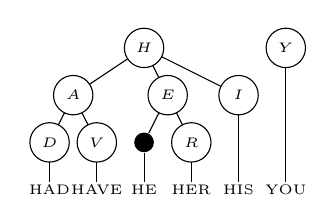
\begin{tikzpicture}[
			state/.style = { circle, top color = white, bottom color = white, draw, black, text = black, minimum width = 0.5 cm, font = \tiny, inner sep=0pt, outer sep=0pt },
			comp/.style = {font = \tiny, inner sep=0.5pt, outer sep=0.5pt},
			end/.style = { circle, fill, color = black, inner sep=0pt, minimum width = 0.25 cm }
			]
			
			\def\oneUnit{0.6cm}
			
			\node[state] (H) at (0*\oneUnit,0*\oneUnit) {$H$};
			\node[state] (Y) at (3*\oneUnit,0*\oneUnit) {$Y$};
			
			\node[state] (A) at (-1.5*\oneUnit,-1*\oneUnit) {$A$};
			\node[state] (E) at (0.5*\oneUnit,-1*\oneUnit) {$E$};
			\node[state] (I) at (2*\oneUnit,-1*\oneUnit) {$I$};
			
			\node[state] (D) at (-2*\oneUnit,-2*\oneUnit) {$D$};
			\node[state] (V) at (-1*\oneUnit,-2*\oneUnit) {$V$};
			\node[end] (HEend) at (0*\oneUnit,-2*\oneUnit) {};
			\node[state] (R) at (1*\oneUnit,-2*\oneUnit) {$R$};
			
			\node[comp] (compHAD) at (-2*\oneUnit,-3*\oneUnit) {\rotatedBox{HAD}};
			\node[comp] (compHAVE) at (-1*\oneUnit,-3*\oneUnit) {\rotatedBox{HAVE}};
			\node[comp] (compHE) at (0*\oneUnit,-3*\oneUnit) {\rotatedBox{HE}};
			\node[comp] (compHER) at (1*\oneUnit,-3*\oneUnit) {\rotatedBox{HER}};
			\node[comp] (compHIS) at (2*\oneUnit,-3*\oneUnit) {\rotatedBox{HIS}};
			\node[comp] (compYOU) at (3*\oneUnit,-3*\oneUnit) {\rotatedBox{YOU}};
			
			\path (H) edge [] (A);
			\path (H) edge [] (E);
			\path (H) edge [] (I);
			\path (Y) edge [] (compYOU);
			
			\path (A) edge [] (D);
			\path (A) edge [] (V);
			\path (E) edge [] (HEend);
			\path (E) edge [] (R);
			
			\path (D) edge [] (compHAD);
			\path (V) edge [] (compHAVE);
			\path (HEend) edge [] (compHE);
			\path (R) edge [] (compHER);
			\path (I) edge [] (compHIS);
			\end{tikzpicture}
			\subcaption{Fragment lasu o skróconej strukturze zaproponowanej przez Knuth'a. Każdy węzeł posiadający pojedyncze dziecko może zawierać więcej niż jeden znak (w tym znak końca słowa). Takimi wyjątkowymi węzłami są te zawierające znaki: \texttt{D}, \texttt{V}, \texttt{R}, \texttt{I} oraz \texttt{Y}. Taki las skróconych drzew \emph{Trie} często nazywany jest lasem drzew \emph{Patricia}. Różni się to od definicji drzewa \emph{Patricia} przyjętej przez Knuth'a, gdyż korzysta ona tylko z jednej jej cechy.}\label{fig:SkroconeDrzewoTrie}
		\end{subfigure}
		\begin{subfigure}{0.35\textwidth}
			\centering
			\begin{tikzpicture}[
			>={Stealth[inset=0pt,length=4pt, angle'=80,round]},
			state/.style = { circle, top color = white, bottom color = white, draw, black, text = black, minimum width = 0.5 cm, font = \tiny, inner sep=0pt, outer sep=0pt },
			comp/.style = {font = \tiny, inner sep=0.5pt, outer sep=0.5pt},
			end/.style = { circle, fill, color = black, inner sep=0pt, minimum width = 0.25 cm }
			]
			
			\def\oneUnit{0.6cm}
			
			\node[state] (H) at (0*\oneUnit,0*\oneUnit) {$H$};
			\node[state] (I1) at (3*\oneUnit,0*\oneUnit) {$I$};
			
			\node[state] (A) at (-1.5*\oneUnit,-1*\oneUnit) {$A$};
			\node[state] (E1) at (0.5*\oneUnit,-1*\oneUnit) {$E$};
			\node[state] (I2) at (2*\oneUnit,-1*\oneUnit) {$I$};
			
			\node[state] (D) at (-2*\oneUnit,-2*\oneUnit) {$D$};
			\node[state] (V) at (-1*\oneUnit,-2*\oneUnit) {$V$};
			\node[end] (HEend) at (0*\oneUnit,-2*\oneUnit) {};
			\node[state] (R) at (1*\oneUnit,-2*\oneUnit) {$R$};
			\node[state] (S) at (2*\oneUnit,-2*\oneUnit) {$S$};
			
			\node[end] (HADend) at (-2*\oneUnit,-3*\oneUnit) {};
			\node[state] (E2) at (-1*\oneUnit,-3*\oneUnit) {$E$};
			\node[end] (HERend) at (1*\oneUnit,-3*\oneUnit) {};
			\node[end] (HISend) at (2*\oneUnit,-3*\oneUnit) {};
			
			\node[end] (HAVEend) at (-1*\oneUnit,-4*\oneUnit) {};
			
			\node[comp] (compHAD) at (-2*\oneUnit,-5*\oneUnit) {\rotatedBox{HAD}};
			\node[comp] (compHAVE) at (-1*\oneUnit,-5*\oneUnit) {\rotatedBox{HAVE}};
			\node[comp] (compHE) at (0*\oneUnit,-5*\oneUnit) {\rotatedBox{HE}};
			\node[comp] (compHER) at (1*\oneUnit,-5*\oneUnit) {\rotatedBox{HER}};
			\node[comp] (compHIS) at (2*\oneUnit,-5*\oneUnit) {\rotatedBox{HIS}};
			
			\path (H) edge [->, dashed] node[above] {\scriptsize \texttt{RLINK}} (I1);
			
			\path (H) edge [->] node[left = 0.3cm, above] {\scriptsize \texttt{LLINK}} (A);
			\path (A) edge [->] (E1);
			\path (A) edge [->] (D);
			\path (E1) edge [->] (I2);
			\path (E1) edge [->] (HEend);
			\path (I2) edge [->] (S);
			
			\path (D) edge [->] (V);
			\path (D) edge [->] (HADend);
			\path (V) edge [->] (E2);
			\path (HEend) edge [] (compHE);
			\path (HEend) edge [->] (R);
			\path (R) edge [->] (HERend);
			\path (S) edge [->] (HISend);
			
			\path (HADend) edge [] (compHAD);
			\path (E2) edge [->] (HAVEend);
			\path (HERend) edge [] (compHER);
			\path (HISend) edge [] (compHIS);
			
			\path (HAVEend) edge [] (compHAVE);
			
			\end{tikzpicture}			
			\subcaption{Fragment drzewa binarnego odzwierciedlającego strukturę lasu drzew \emph{Trie} z figury~\ref{fig:CompleteTrieForest}}\label{fig:BinarneDrzewoTrie}
		\end{subfigure}
		\caption{Porównanie fragmentów: \protect\subref{fig:SkroconeDrzewoTrie} skróconego lasu \emph{Trie} oraz \protect\subref{fig:BinarneDrzewoTrie} \emph{binarnego drzewa}. Oba rysunki zasięgnięte są z książki Knuth'a \cite{KnuthsTheArtOfComputerProgramming3}.}
	\end{figure}
	
	Skrócona budowa lasu \emph{Trie} charakteryzuje się mniejszymi wymogami pamięciowymi, ale bardziej skomplikowanym mechanizmem przetwarzania danych -- jak na przykład wkładaniem nowych obiektów czy kasowaniem istniejących.\newline
	
	Reprezentacja w postaci drzewa binarnego wiążę się z jego przeszukiwaniem poprzez porównywanie znaku argumentu ze znakiem w drzewie. Jeżeli znaki sobie nie odpowiadają to podążamy za \emph{RLINK} -- wskaźnikiem oznaczającym prawą gałąź, a gdy pasują do siebie przechodzimy do węzła wskazanego przez \emph{LLINK} -- wskaźnikiem oznaczającym lewą gałąź. Postępujemy tak oczywiście od pierwszego znaku argumentu do ostatniego. 
	
	\ifsourcematerial	
	\begin{displayquote}
		\color{ao(english)}
		\underline{\textbf{FRAGMENT TŁUMACZONY:}} \newline
		
		in place of the “H” tree in Fig. 31. This representation requires more storage, but it makes the processing of variable-length data especially easy. If we use two
		link fields per character, dynamic insertions and deletions can be handled in a
		simple manner.
		
		If we use the normal way of representing trees as binary trees, (1) becomes
		the binary tree
		
		\elide Dokończenie schematu lasu de la Briandais'a w postaci drzewa binarnego. \elide
		
		In the representation of the full forest, Fig. 31, we would also have a pointer
		leading to the right from to its neighboring root .) The search in this binary
		tree proceeds by comparing a character of the argument to the character in the
		tree, and following \texttt{RLINK}s until finding a match; then the \texttt{LLINK} is taken and
		we treat the next character of the argument in the same way.
		
	\end{displayquote}
	\fi
	
	Takie przeszukiwanie jest określane przez Knuth'a \emph{rozgałęzieniem ze względu na porównanie równe-nierówne} (ang. \emph{equal-unequal branching}), które zostaje wykorzystane w miejsce \emph{rozgałęzienia mniejsze-większe} (ang. \emph{less-greater branching}).
	
	\subsubsection{Złożoność czasowa i pamięciowa oraz przeznaczenie i możliwe modyfikacje w ich kontekście}\label{sec:LasTriePrzeszukiwanieZlozonoscCzasowaIPamieciowaIPrzeznaczenie}
	
	Wynikająca z tego charakterystyka złożoności obliczeniowej mówi o minimalnej ilości porównań wynoszącej: 
	
	\begin{equation}\label{eq:zlozonoscCzasowaZrandomizowanaDrzewTrie}
	lg(N) = log_2(N)
	\end{equation}
	gdzie
	\begin{eqwhere}[2cm]
		\item[$N$] ilość kluczy
	\end{eqwhere}
	
	\ifsourcematerial	
	\begin{displayquote}
		\color{ao(english)}
		\underline{\textbf{FRAGMENT TŁUMACZONY:}} \newline
		With such a binary tree, we are more or less doing a search by comparison,
		with equal-unequal branching instead of less-greater branching. The elementary
		theory of Section 6.2.1 tells that we must make at least lg N comparisons, on the
		average, to distinguish between N keys; 
	\end{displayquote}
	\fi
	
	Przeszukiwanie drzewa przedstawionego przez rysunek~\ref{fig:CompleteTrieTree} średnio wymaga co~najmniej takiej samej ilości porównań jak w przypadku przeszukiwania drzewa binarnego. Jednak w drzewie \emph{Trie} z tabeli~\ref{tab:trieTreeFor31MostCommonEnglishWords} z jednego węzła może wychodzić $M$ rozgałęzień.\newline Dla dużych ilości kluczy $N$ i dla danych zrandomizowanych skutkuje to czasem przeszukiwania określonych zależnością:
	
	\begin{equation}
	log_M(N) = \frac{lg(N)}{lg(M)}
	\end{equation}
	gdzie
	\begin{eqwhere}[2cm]
		\item[$N$] ilość kluczy
		\item[$M$] ilość gałęzi wychodzących z każdego węzła, znaków rozważanego alfabetu 
	\end{eqwhere}
	
	Knuth zwraca dodatkowo uwagę na fakt, iż nazywana przez niego ,,czysta`` struktura \emph{Trie} -- jak ta zaprezentowana w przypadku omawianego Algorytmu T w sekcji~\ref{sec:AlgorytmT} -- wymaga około
	
	\begin{equation}
	\frac{N}{ln(M)}
	\end{equation}
	
	węzłów by rozróżnić $N$ losowych kluczy podanych jako argument danych wejściowych, a co za tym idzie całkowita ilość pamięci jest proporcjonalna do wzoru:
	
	\begin{equation}
	\frac{MN}{ln(M)}
	\end{equation}
	
	\ifsourcematerial
	\begin{displayquote}
		\color{ao(english)}
		\underline{\textbf{FRAGMENT TŁUMACZONY:}} \newline
		
		the average number of tests made when searching a tree like that of \textbf{Fig. 31} must be at least as many as we make when
		doing a binary search using the techniques of \textbf{Section 6.2}.
		On the other hand, the trie in \textbf{Table 1} is capable of making an M-way branch
		all at once; we shall see that the average search time for large N involves only
		about 
		
		\begin{equation}
		log_M(N) = lg(N)/lg(M)
		\end{equation}
		
		iterations, if the input data is random. We shall also see that a “pure” trie scheme
		like that in Algorithm T requires a total of approximately N/ln M nodes to
		distinguish between N random inputs; hence the total amount of space is
		proportional to MN/ln M.
	\end{displayquote}
	\fi
	
	Wnioskiem wyciąganym z tej analizy przez Knuth'a jest fakt, że użycie struktury \emph{Trie} zaczyna mieć sens tylko w kilku pierwszych poziomach drzewa. Proponuje on wymieszanie dwóch strategii -- używanie \emph{Trie} przez kilka pierwszych znaków argumentu przeszukiwania, a potem zmianę struktury. Knuth przytacza technikę opisaną przez E. H. Sussenguth, Jr. [CACM 6 (1963), 272–279], gdzie następuje zmiana strategii, gdy pozostaje 6 lub mniej możliwych kluczy na przechodzenie przez krótką listę pozostałych kluczy. Skutkuje to zmniejszeniem ilości węzłów \emph{Trie} sześciokrotnie bez znaczących zmian czasu wykonywania przeszukiwania.
	
	\ifsourcematerial
	\begin{displayquote}
		\color{ao(english)}
		\underline{\textbf{FRAGMENT TŁUMACZONY:}} \newline
		
		From these considerations it is clear that the trie idea pays off only in the
		first few levels of the tree. We can get better performance by mixing two
		strategies, using a trie for the first few characters and then switching to someother technique. For example, E. H. Sussenguth, Jr. [CACM 6 (1963), 272–279]
		suggested using a character-by-character scheme until we reach part of the tree
		where only, say, six or fewer keys of the file are possible, and then we can
		sequentially run through the short list of remaining keys. We shall see that this
		mixed strategy decreases the number of trie nodes by roughly a factor of six,
		without substantially changing the running time.
	\end{displayquote}
	\fi
	
	Knuth w swojej książce wyróżnia jeszcze dwa ciekawe pomysły na optymalizację algorytmu zaproponowane przez innych autorów. 
	Pierwszym z nich jest sposób na przetrzymywanie dużych i rosnących drzew w zewnętrznej pamięci autorstwa S. Y. Berkovich w Doklady Akademii Nauk SSSR 202 (1972), 298 - 299 [English translation in Soviet Physics–Doklady 17 (1972), 20–21]. 
	Drugim jest uwaga z pracy T.N. Tubra [CACM 25 (1982), 522–526], dotycząca tego, że czasem najwygodniej jest szukać po ilości kluczy zmiennej argumentu przeszukiwania, posiadając po jednym drzewie lub drzewie \emph{Trie} na każdą długość.
	
	\ifsourcematerial
	\begin{displayquote}
		\color{ao(english)}
		\underline{\textbf{FRAGMENT TŁUMACZONY:}} 
		
		An interesting way to store large, growing tries in external memory was
		suggested by S. Y. Berkovich in Doklady Akademii Nauk SSSR 202 (1972), 298–
		299 [English translation in Soviet Physics–Doklady 17 (1972), 20–21].
		T. N. Turba [CACM 25 (1982), 522–526] points out that it is sometimes
		most convenient to search for variable-length keys by having one search tree or
		trie for each different length.
	\end{displayquote}
	\fi
	
	\subsection{Przypadek binarny -- Przeszukiwanie cyfrowe drzewa oraz wstawianie}\label{sec:PrzypadekBinarnyPrzeszukiwanieCyfroweDrzewaOrazWstawianie}
	
	Przypadek binarny to pojęcie, którego Knuth używa do opisania rodzaju drzewa binarnego, czyli drzewa \emph{M-ary} dla $M=2$, w którym przeszukiwanie polega na skanowaniu bitów po kolei. Metoda przeszukiwania takiego drzewa nazywana jest \emph{przeszukiwaniem drzewa cyfrowego} i została opracowana przez E. G. Coffman	and J. Eve [CACM 13 (1970), 427–432, 436]. W węzłach drzewa przetrzymywane są pełne klucze, czyli całe słowa. O tym, którą gałąź drzewa należy wybrać, aby znaleźć odpowiednie słowo, decyduje reprezentacja binarna poszczególnych znaków argumentu przeszukiwania.\newline
	
	Rysunek~\ref{fig:DigitalSearchTree} przedstawia drzewo binarne, nazywane też drzewem przeszukiwania cyfrowego lub drzewem cyfrowym, stworzone poprzez wstawianie słów w kolejności zależnej od ich częstotliwości występowania. Najpopularniejsze słowa są umieszczone jak najbliżej korzenia drzewa, a mniej popularne głębiej, ale nadal w zgodności z wcześniej opisaną metodą wyboru gałęzi. \newline
	
	\begin{figure}[htb]
		\caption{Schemat drzewa przeszukiwania cyfrowego dla 31 najpopularniejszych słów angielskich. Drzewo przeszukujemy odwołując się do wartości binarnej słowa szukanego i analizujemy każdy jego bit zaczynając od lewej strony. Dla $0$ idziemy do lewego dziecka a dla $1$ do prawego. Rysunek zasięgnięty jest z książki Knuth'a \cite{KnuthsTheArtOfComputerProgramming3}.}\label{fig:DigitalSearchTree}
		\centering
		\begin{tikzpicture}[
		>={Stealth[inset=0pt,length=4pt, angle'=45,round]},
		state/.style = { rectangle, rounded corners, top color = white, bottom color = white, draw, black, text = black, minimum width = 0.75 cm, minimum height = 0.5cm, font = \tiny, inner sep=0.05cm, outer sep=0.05cm },
		comp/.style = {font = \tiny, inner sep=0.5pt, outer sep=0.5pt},
		end/.style = { circle, fill, color = black, inner sep=0pt, minimum width = 0.25 cm }
		]
		
		\def\oneUnit{0.75cm}
		
		\node[state] (THE) at (0*\oneUnit,0*\oneUnit) {$THE$};
		
		\node[state] (AND) at (-5*\oneUnit,-1*\oneUnit) {$AND$};
		\node[state] (OF) at (5*\oneUnit,-1*\oneUnit) {$OF$};			
		
		\node[state] (A) at (-7.5*\oneUnit,-2*\oneUnit) {$A$};
		\node[state] (IN) at (-2.5*\oneUnit,-2*\oneUnit) {$IN$};
		\node[state] (TO) at (2.5*\oneUnit,-2*\oneUnit) {$TO$};
		\node[state] (WITH) at (7.5*\oneUnit,-2*\oneUnit) {$WITH$};
		
		\node[state] (AS) at (-8.75*\oneUnit,-3*\oneUnit) {$AS$};
		\node[state] (FOR) at (-6.25*\oneUnit,-3*\oneUnit) {$FOR$};
		\node[state] (IS) at (-3.75*\oneUnit,-3*\oneUnit) {$IS$};
		\node[state] (NOT) at (-1.25*\oneUnit,-3*\oneUnit) {$NOT$};
		\node[state] (ON) at (1.25*\oneUnit,-3*\oneUnit) {$ON$};
		\node[state] (THAT) at (3.75*\oneUnit,-3*\oneUnit) {$THAT$};
		\node[state] (WAS) at (6.25*\oneUnit,-3*\oneUnit) {$WAS$};
		\node[state] (YOU) at (8.75*\oneUnit,-3*\oneUnit) {$YOU$};
		
		\node[state] (ARE) at (-10*\oneUnit,-4*\oneUnit) {$ARE$};
		\node[state] (BE) at (-7.5*\oneUnit,-4*\oneUnit) {$BE$};
		\node[state] (FROM) at (-5.75*\oneUnit,-4*\oneUnit) {$FROM$};
		\node[state] (I) at (-4.25*\oneUnit,-4*\oneUnit) {$I$};
		\node[state] (OR) at (0*\oneUnit,-4*\oneUnit) {$OR$};
		\node[state] (THIS) at (5*\oneUnit,-4*\oneUnit) {$THIS$};
		\node[state] (WHICH) at (7.5*\oneUnit,-4*\oneUnit) {$WHICH$};
		
		\node[state] (AT) at (-9.5*\oneUnit,-5*\oneUnit) {$AT$};
		\node[state] (BY) at (-8*\oneUnit,-5*\oneUnit) {$BY$};
		\node[state] (HIS) at (-5*\oneUnit,-5*\oneUnit) {$HIS$};
		\node[state] (IT) at (-3.5*\oneUnit,-5*\oneUnit) {$IT$};
		
		\node[state] (BUT) at (-7.5*\oneUnit,-6*\oneUnit) {$BUT$};
		\node[state] (HE) at (-5.75*\oneUnit,-6*\oneUnit) {$HE$};
		
		\node[state] (HAVE) at (-6.5*\oneUnit,-7*\oneUnit) {$HAVE$};
		
		\node[state] (HAD) at (-7.25*\oneUnit,-8*\oneUnit) {$HAD$};
		\node[state] (HER) at (-5.75*\oneUnit,-8*\oneUnit) {$HER$};
		
		\path (THE) edge [->] node[above = -0.25 cm] {\tiny \contour{white}{$0$}} (AND);
		\path (THE) edge [->] node[above = -0.25 cm] {\tiny \contour{white}{$1$}} (OF);
		
		\path (AND) edge [->] node[above = -0.25 cm] {\tiny \contour{white}{$0$}} (A);			
		\path (AND) edge [->] node[above = -0.25 cm] {\tiny \contour{white}{$1$}} (IN);
		\path (OF) edge [->] node[above = -0.25 cm] {\tiny \contour{white}{$0$}} (TO);
		\path (OF) edge [->] node[above = -0.25 cm] {\tiny \contour{white}{$1$}} (WITH);
		
		\path (A) edge [->] node[above = 0.1 cm, left] {\tiny \contour{white}{$0$}} (AS);
		\path (A) edge [->] node[above = 0.1 cm, right] {\tiny \contour{white}{$1$}} (FOR);
		\path (IN) edge [->] node[above = 0.1 cm, left] {\tiny \contour{white}{$0$}} (IS);
		\path (IN) edge [->] node[above = 0.1 cm, right] {\tiny \contour{white}{$1$}} (NOT);
		\path (TO) edge [->] node[above = 0.1 cm, left] {\tiny \contour{white}{$0$}} (ON);
		\path (TO) edge [->] node[above = 0.1 cm, right] {\tiny \contour{white}{$1$}} (THAT);
		\path (WITH) edge [->] node[above = 0.1 cm, left] {\tiny \contour{white}{$0$}} (WAS);
		\path (WITH) edge [->] node[above = 0.1 cm, right] {\tiny \contour{white}{$1$}} (YOU);
		
		\path (AS) edge [->] node[above = 0.1 cm, left] {\tiny \contour{white}{$0$}} (ARE);
		\path (AS) edge [->] node[above = 0.1 cm, right] {\tiny \contour{white}{$1$}} (BE);
		\path (FOR) edge [->] node[yshift = 0.05 cm, xshift = 0.35 cm] {\tiny \contour{white}{$1$}} (FROM);
		\path (IS) edge [->] node[yshift = 0.05 cm, xshift = -0.35 cm] {\tiny \contour{white}{$0$}} (I);
		\path (ON) edge [->] node[above = 0.1 cm, left] {\tiny \contour{white}{$0$}} (OR);
		\path (THAT) edge [->] node[above = 0.1 cm, right] {\tiny \contour{white}{$1$}} (THIS);
		\path (WAS) edge [->] node[above = 0.1 cm, right] {\tiny \contour{white}{$1$}} (WHICH);
		
		
		\path (ARE) edge [->] node[yshift = 0.05 cm, xshift = 0.35 cm] {\tiny \contour{white}{$1$}} (AT);
		\path (BE) edge [->] node[yshift = 0.05 cm, xshift = -0.35 cm] {\tiny \contour{white}{$0$}} (BY);
		\path (I) edge [->] node[yshift = 0.05 cm, xshift = -0.35 cm] {\tiny \contour{white}{$0$}} (HIS);
		\path (I) edge [->] node[yshift = 0.05 cm, xshift = 0.35 cm] {\tiny \contour{white}{$1$}} (IT);
		
		\path (BY) edge [->] node[yshift = 0.05 cm, xshift = 0.35 cm] {\tiny \contour{white}{$1$}} (BUT);
		\path (HIS) edge [->] node[yshift = 0.05 cm, xshift = -0.35 cm] {\tiny \contour{white}{$0$}} (HE);
		
		\path (HE) edge [->] node[yshift = 0.05 cm, xshift = -0.35 cm] {\tiny \contour{white}{$0$}} (HAVE);
		
		\path (HAVE) edge [->] node[yshift = 0.05 cm, xshift = -0.35 cm] {\tiny \contour{white}{$0$}} (HAD);
		\path (HAVE) edge [->] node[yshift = 0.05 cm, xshift = 0.35 cm] {\tiny \contour{white}{$1$}} (HER);
		\end{tikzpicture}
	\end{figure}
	\newpage
    Jeżeli chcielibyśmy w tym drzewie znaleźć słowo \texttt{WHICH}, to wchodząc do drzewa, porównalibyśmy cały argument przeszukiwania z całym kluczem węzła \texttt{THE}. Nie znajdując dopasowania, musielibyśmy wybrać jedną z gałęzi. Skoro pierwszym bitem reprezentacji binarnej poszukiwanego słowa jest $1$ musimy wybrać gałąź prawą. Ponownie należy porównać ze sobą całe słowa węzła i argumentu przeszukiwania -- \texttt{WHICH} i \texttt{OF} -- wybrać gałąź prawą ze względu na drugi bit równy $1$. Proces powtarzamy dla węzła \texttt{WITH}, wybieramy gałąź lewą dla trzeciego bitu równego $0$ i ponownie porównujemy z \texttt{WAS}. Ostatni raz analizujemy bit -- tym razem czwarty -- równy $1$ wybierając gałąź prawą. Skoro nie ma już dalszych gałęzi, ostatnie porównanie decyduje o tym, czy dane słowo znajduje się w naszym drzewie, czy jednak go tam nie ma. Na szczęście tym razem słowa argumentu przeszukiwania i węzła pasują do siebie, czyli udało nam się znaleźć poszukiwane słowo. Jeżeli jednak tak by się nie stało, to w przypadku wstawiania musielibyśmy stworzyć nowy węzeł zawierający pełny klucz argumentu przeszukiwania, a następnie wybrać odpowiednią gałąź na podstawie piątego bitu, równego $0$ -- czyli gałąź lewą -- która wskazywałaby na nowo stworzony węzeł.\newline
	
	Tabela~\ref{tab:MixBitReprezentationFor31MostCommonEnglishWords} przestawia reprezentację binarną wszystkich słów w drzewie zgodnie z kodowaniem znaków maszyny \emph{MIX} Knuth'a~\cite{wikiMix}. Słowa ułożone są w kolejności występowania w drzewie, czytane od lewej do prawej, poziom po poziomie. Korzeniem jest najczęściej występujące słowo \texttt{THE}, którego częstotliwość występowania wynosi 15586. Następnym słowem w tablicy jest \texttt{AND}, choć \texttt{OF} ma od niego większą częstotliwość występowania. Jest to związane ze strukturą drzewa, które budowane jest w oparciu o reprezentację binarną poszczególnych słów. Choć częstotliwość występowania jest priorytetowym kryterium w kontekście tworzenia drzewa przeszukiwania cyfrowego, to ze względu na jego charakterystykę, nie zawsze najczęściej występujące słowa będą znajdowały się wysoko w tabeli.\newline 	
	
	\ifsourcematerial
	\begin{displayquote}
		\color{ao(english)}
		\underline{\textbf{FRAGMENT TŁUMACZONY:}} \newline 
		In order to provide binary data for this illustration, the
		words have been expressed in \texttt{MIX}
		character code, and the codes have been
		converted into binary numbers with 5 bits per byte. Thus, the word \texttt{WHICH}
		is represented as the bit sequence 11010 01000 01001 00011 01000. 
		
		To search for this word \texttt{WHICH}
		in Fig. 32, we compare it first with the word \texttt{THE}
		at the root of the tree. Since there is no match and since the first bit of \texttt{WHICH}
		is 1, we move to the right and compare with \texttt{OF}. Since there is no match
		and since the second bit of \texttt{WHICH}
		is 1, we move to the right and compare with \texttt{WITH}
		; and so on. Alphabetic order of the keys in a digital search tree no longer
		corresponds to symmetric order of the nodes.
		
		\color{graphcolorblue}
		\href{https://esolangs.org/wiki/MIX_(Knuth)#General}{Knuth's MIX mechine and character codes}
	\end{displayquote}
	\fi
	
	\begin{table}
		\centering
		\begin{threeparttable}
			\caption{Tablica 31 najpopularniejszych angielskich słów, ich częstotliwości wystąpień oraz reprezentacji binarnej w maszynie Knuth'a \emph{MIX}. Kolumna zawierająca reprezentację dziesiętną jest wynikiem zamiany poszczególnych znaków w słowie na wartości, które Knuth przypisuje znakom w swojej maszynie \emph{MIX}~\cite{wikiMix}. Np. dla litery \texttt{T} wynosi ona 23, dla \texttt{H} -- 8, a dla \texttt{E} -- 5. Reprezentacja binarna jest tworzona na podstawie zamiany liczb z reprezentacji dziesiętnej na wartości binarne. Tablica zasięgnięta jest z książki Knuth'a \cite{KnuthsTheArtOfComputerProgramming3}.}\label{tab:MixBitReprezentationFor31MostCommonEnglishWords}
			
			{ \small
				\begin{tabularx}{0.86\textwidth}{C{3}|C{6}|C{6}|C{14}|}
					\textbf{Słowo} & \textbf{Częstotliwość występowania} & \textbf{Reprezentacja dziesiętna} & \textbf{Reprezentacja binarna} \\
					\hline \hline
					THE 	& 15586 	& 23 8 5 		& 10111 01000 00101 \\
					AND 	& 7638 		& 1 15 4 		& 00001 01111 00100 \\
					OF 		& 9767		& 16 6 			& 10000 00110 \\
					A 		& 5074 		& 1 			& 00001 \\
					IN 		& 4312 		& 9 15 			& 01001 01111 \\
					TO 		& 5739 		& 23 16 		& 10111 10000 \\
					WITH 	& 1849 		& 26 9 23 8 	& 11010 01001 10111 01000 \\
					AS 		& 1853 		& 1 22 			& 00001 10110 \\
					FOR 	& 1869 		& 6 16 19 		& 00110 10000 10011 \\
					IS 		& 2509 		& 9 22 			& 01001 10110 \\
					NOT 	& 1496 		& 15 16 23 		& 01111 10000 10111 \\
					ON 		& 1155 		& 16 15 		& 10000 01111 \\
					THAT 	& 3017 		& 23 8 1 23 	& 10111 01000 00001 10111 \\
					WAS 	& 1761 		& 26 1 22 		& 11010 00001 10110 \\
					YOU 	& 1336 		& 28 16 24 		& 11100 10000 11000 \\
					ARE 	& 1222 		& 1 19 5 		& 00001 10011 00101 \\
					BE 		& 1535 		& 2 5 			& 00010 00101 \\
					FROM 	& 1039 		& 6 19 16 14 	& 00110 10011 10000 01110 \\
					I 		& 2292 		& 9 			& 01001 \\
					OR 		& 1101 		& 16 19 		& 10000 10011 \\
					THIS 	& 1021 		& 23 8 9 22 	& 10111 01000 01001 10110 \\
					WHICH 	& 1291 		& 26 8 9 3 8 	& 11010 01000 01001 00011 01000 \\
					AT 		& 1053 		& 1 23 			& 00001 10111 \\
					BY 		& 1392 		& 2 28 			& 00010 11100 \\
					HIS 	& 1732 		& 8 9 22 		& 01000 01001 10110 \\
					IT 		& 2255 		& 9 23 			& 01001 10111 \\
					BUT 	& 1379 		& 2 24 23 		& 00010 11000 \\
					HE 		& 1727 		& 8 5 			& 01000 00101 \\
					HAVE 	& 1344 		& 8 1 25 5 		& 01000 00001 11001 00101 \\ 
					HAD 	& 1062 		& 8 1 4 		& 01000 00001 00100 \\
					HER 	& 1093 		& 8 5 19 		& 01000 00101 10011 \\
				\end{tabularx} 
			}
		\end{threeparttable}
	\end{table}
	
	\subsubsection{Algorytm D -- Wstawianie}\label{sec:AlgorytmD}
	
	\textbf{Założenia:}
	
	Dana jest tablica rekordów tworzących binarne drzewo opisane tablicą~\ref{fig:DigitalSearchTree} oraz tablicą~\ref{tab:MixBitReprezentationFor31MostCommonEnglishWords}. Algorytm przeszukuje drzewo w celu znalezienia danego argumentu $K$. Jeżeli $K$ nie znajduje się w tablicy, nowy węzeł zawierający argument $K$ zostanie dodany do drzewa w odpowiednie miejsce. Zakładamy, że drzewo jest niepuste i każdy z węzłów posiada \emph{KEY}, \emph{LLINK} -- będący wskaźnikiem, reprezentującym lewą gałąź - oraz \emph{RLINK} -- również będący wskaźnikiem, reprezentującym prawą gałąź.
	
	\begin{enumerate}
		\item \textbf{Inicjalizacja} \newline 
		Ustaw $P$ -- nasze odniesienie do obecnie przetwarzanego węzła -- tak, aby wskazywało na korzeń drzewa. \newline
		Ustaw $K`$ -- nieprzetworzone bity reprezentacji bitowej argumentu przeszukiwania -- na reprezentacje bitową całego argumentu przeszukiwania $K$.
		\item \textbf{Porównanie} 
		\begin{enumerate}
			\item Jeżeli $K`$ jest \emph{KEY}($P$) (kluczem $P$) -- zakończ przeszukiwanie z powodzeniem.
			\item W przeciwnym wypadku: \newline
			Ustaw $b$ na początkowy bit $K`$, \newline
			Przesuń $K`$ o jeden bit w lewo, czyli usuń najbardziej znaczący bit, przesuwając pozostałe bity oraz dokładając na puste miejsce, najmniej znaczącego bitu~$0$~\cite{inteviewCakeJavaBitShifting}.
			\begin{enumerate}
				\item Jeżeli $b$ $=0$ -- idź do punktu 3.
				\item W przeciwnym wypadku -- idź do punktu 4.
			\end{enumerate}
		\end{enumerate}
		\item \textbf{Ruch w lewo} 
		\begin{enumerate}
			\item Jeżeli \emph{LLINK($P$)} wskazuje na istniejący węzeł, nie jest pustym, \emph{null} wskaźnikiem: \newline
			Ustaw $P$ na \emph{LLINK($P$)}, \newline
			Idź do punktu 2.
			\item W przeciwnym wypadku -- idź do punktu 5.
		\end{enumerate}
		\item \textbf{Ruch w prawo} 
		\begin{enumerate}
			\item Jeżeli \emph{RLINK($P$)} wskazuje na istniejący węzeł, nie jest pustym, \emph{null} wskaźnikiem: \newline
			Ustaw $P$ na \emph{RLINK($P$)}, \newline
			Idź do punktu 2.
			\item W przeciwnym wypadku -- idź do punktu 5. 
		\end{enumerate}
		\item \textbf{Wstawienie do drzewa} \newline 
		Stwórz nowy węzeł $Q$, \newline 
		Ustaw klucz nowego węzła $Q$ na pełen argument przeszukiwania $K$, \newline 
		Ustaw \emph{LLINK($Q$)} oraz \emph{RLINK($Q$)} na \emph{null}.
		\begin{enumerate}
			\item Jeżeli $b$ $=0$ to ustaw \emph{LLINK($P$)} na nowy węzeł $Q$.
			\item W przeciwnym wypadku ustaw \emph{RLINK($P$)} na nowy węzeł $Q$.
		\end{enumerate}
	\end{enumerate}


	\subsubsection{Przeznaczenie}\label{sec:AlgorytmDPrzeznaczenie}
	
	Głównym ograniczeniem tego algorytmu jest wymóg posiadania częstotliwości lub prawdopodobieństwa zapytania o każdy z zawartych w drzewie kluczy. Bez tej informacji struktura nie może być poprawnie zbudowana, gdyż zakłada ona dopasowanie do przypadku użycia. 
	
	W najgorszym wypadku budowa struktury może posiadać najczęściej wyszukiwane klucze oddalone maksymalnie od korzenia drzewa -- tym samym zamiast skracać średni czas wyszukiwania, wydłuża go.
	
	\ifsourcematerial
	\begin{displayquote}
		\color{ao(english)}
		\underline{\textbf{FRAGMENT TŁUMACZONY:}} \newline 
		Algorithm D (Digital tree search and insertion). Given a table of records that
		form a binary tree as described above, this algorithm searches for a given
		argument K. If K is not in the table, a new node containing K is inserted into the
		tree in the appropriate place.
		This algorithm assumes that the tree is nonempty and that its nodes have \texttt{KEY}, ,\texttt{LLINK} and \texttt{RLINK} fields just as in Algorithm 6.2.2T. In fact, the two algorithms are almost identical, as the reader may verify. \newline
		D1. \textbf{[Initialize.]} \newline
		Set \texttt{P} ← \texttt{ROOT};
		Set K` ← K. \newline
		D2. \textbf{[Compare.]} \newline
		If K = \texttt{KEY(P)}: \newline
		\hspace{1cm} The search terminates successfully.
		Otherwise: \newline
		\hspace{1cm} set b to the leading bit of K`, and shift K` left one place \newline
		(thereby removing that bit and introducing a 0 at the right). \newline 
		\hspace{1cm} If b = 0: \newline
		\hspace{2cm} go to D3, \newline
		\hspace{1cm} Otherwise go to D4. \newline
		D3. \textbf{[Move left.]} \newline
		If \texttt{LLINK(P)} $\neq$ $\Lambda$ [$\Lambda$ - null pointer], set \texttt{P} ← \texttt{LLINK(P)} and go back to D2. Otherwise go to D5. \newline
		D4. \textbf{[Move right.]} \newline 
		If \texttt{RLINK(P) $\neq$ $\Lambda$} set \texttt{P} ← \texttt{RLINK(P)} and go back to D2. \newline
		D5. \textbf{[Insert into tree.]} \newline 
		Set Q ← \texttt{AVAIL}, \newline 
		\texttt{KEY(Q)} ← \texttt{K}, \newline
		\texttt{LLINK(Q)} ← RLINK(Q) ← $\Lambda$. \newline
		If b = 0 set \texttt{LLINK(P)} ← Q, otherwise set \texttt{RLINK(P)} ← Q.
		
		\color{graphcolorblue}
		\href{https://www.interviewcake.com/concept/java/bit-shift}{Bit shifting}
	\end{displayquote}
	\fi
	
	\subsection{Drzewo \emph{Patricia} -- N-węzłowe drzewo przeszukiwań binarnej reprezentacji kluczy}\label{sec:DrzewoPatricia}
	
	Rozszerzeniem algorytmu~\ref{sec:AlgorytmD} z binarnego na przypadek przeszukiwania cyfrowego drzewa \emph{M-ary}, dla dowolnego $M \geq 2$ jest opracowana przez Donald R. Morrison [JACM 15 (1968), 514–534]~\cite{PatriciaDonaldRMorrison} metoda ``Patricia`` (ang. \emph{Practical Algorithm To Retrieve Information Coded In Alphanumeric}). Bardzo podobny algorytm został opublikowany w prawie tym samym czasie w Niemczech przez G. Gwehenberger, Elektronische Rechenanlagen 10 (1968), 223–226. \emph{Patricia} jest to metoda tworzenia $N$-węzłowych drzew przeszukiwań oparta o binarną reprezentację kluczy, bez potrzeby przechowywania kluczy w węzłach. Jest ona szczególnie przystosowana dla długich, różnej długości kluczy -- takich jak tytuły czy frazy zawarte w dużych zbiorach plikowych. 
	
	\ifsourcematerial
	\begin{displayquote}
		\color{ao(english)}
		\underline{\textbf{FRAGMENT TŁUMACZONY:}} \newline 
		
		Although the tree search of Algorithm 6.2.2T is inherently binary, it is not
		difficult to see that the present algorithm could be extended to an M-ary digital
		search for any M >= 2 (see exercise 13). \newline
		
		Donald R. Morrison [JACM 15 (1968), 514–534] has discovered a very
		pretty way to form N-node search trees based on the binary representation of
		keys, without storing keys in the nodes. His method, called “Patricia” (Practical
		Algorithm To Retrieve Information Coded In Alphanumeric), is especially
		suitable for dealing with extremely long, variable-length keys such as titles or
		phrases stored within a large bulk file. A closely related algorithm was published
		at almost exactly the same time in Germany by G. Gwehenberger, Elektronische
		Rechenanlagen 10 (1968), 223–226. \newline
	\end{displayquote} 
	\fi
	
	Zamysłem metody \emph{Patricia} jest stworzenie binarnego drzewa, unikając tworzenia węzłów z jedną krawędzią wychodzącą, z jednym dzieckiem -- czyli takich gałęzi, które nie są rozgałęzieniami, które nie powodują zawężenia ilości możliwych do podjęcia ścieżek, a~ich jedyną funkcją jest przesunięcie obecnie analizowanego przypadku o jeden do przodu. Ominięcie takich przypadków jest osiągane przez zawarcie w każdym węźle numeru bitów, które należy pominąć przed przeprowadzeniem testu na następnym.
	
	\ifsourcematerial
	\begin{displayquote}
		\color{ao(english)}
		\underline{\textbf{FRAGMENT TŁUMACZONY:}} \newline 
		
		Patricia’s basic idea is to build a binary trie, but to avoid one-way branching
		by including in each node the number of bits to skip over before making the next
		test. 
	\end{displayquote}
	\fi
	
	Istnieje wiele sposobów wykorzystania tego pomysłu w algorytmie. Knuth przedstawia jeden z nich w następujący sposób. Przygotowujemy tablicę bitów reprezentującą tekst, którą określamy później terminem \emph{TEXT}. Taka tablica zazwyczaj jest długa, więc może być przetrzymywana w postaci pliku. Z powodu wolniejszego dostępu do pliku niż do pamięci RAM należy nałożyć na użytkownika ograniczenie ilości dostępów do tego pliku. Limit ten ustalony zostaje w wysokości jednego odwołania do zawartości pliku przy algorytmie sprawdzania czy dany ciąg znaków jest akceptowany przez nasze drzewo. \newpage
	
	Każdy z kluczy przechowywany wewnątrz tablicy bitów \emph{TEXT} jest określony numerem miejsca w tekście, w którym zaczyna się dany klucz. Należy sobie wyobrazić taki klucz jako ciąg znaków od miejsca startowego danego klucza, aż do końca tekstu. \emph{Patricia} nie jest przeznaczona do znajdywania równości między kluczem, a argumentem przeszukiwania. \emph{Patricia} jedynie odpowiada na pytanie czy istnieje klucz zaczynający się argumentem wejściowym.
	
	Tablica~\ref{tab:PatriciaTreeSourceTextTable} przedstawia przykład zawartości krótkiego pliku w postaci tekstowej. W tym przypadku kluczami przechowywanymi w tablicy \emph{TEXT} są ciągi znaków będące fragmentami tekstu:
	\begin{enumerate}
		\item \texttt{THIS IS THE HOUSE THAT JACK BUILT;}
		\item \texttt{IS THE HOUSE THAT JACK BUILT;}
		\item \texttt{THE HOUSE THAT JACK BUILT;}
		\item \texttt{HOUSE THAT JACK BUILT;}
		\item \texttt{THAT JACK BUILT;}
		\item \texttt{JACK BUILT;}
		\item \texttt{BUILT;}
	\end{enumerate}

	\begin{table}[htb]
		\centering
		\begin{threeparttable}
			\caption{Schemat tablicy przedstawiającej zawartość pliku tekstowego. W wierszu Zawartość przechowujemy poszczególne znaki a w wierszu Numer pozycji, pozycję znaku w pliku, liczoną od lewej i zaczynającą się od numeru 1. Tablica zasięgnięta jest z książki Knuth'a \cite{KnuthsTheArtOfComputerProgramming3}.}\label{tab:PatriciaTreeSourceTextTable}
			
			{ \small
				\begin{tabularx}{\textwidth}{C{4}||C{0.75}|C{0.75}|C{0.75}|C{0.75}|C{0.75}|C{0.75}|C{0.75}|C{0.75}|C{0.75}|C{0.75}|C{0.75}|C{0.75}|C{0.75}|C{0.75}|C{0.75}|C{0.75}|C{0.75}|C{0.75}|C{0.75}|C{0.75}|C{0.75}|C{0.75}|C{0.75}|C{0.75}|C{0.75}|C{0.75}|C{0.75}|C{0.75}|C{0.75}|C{0.75}|C{0.75}|C{0.75}|C{0.75}|C{0.75}}
					\textbf{Zawartość} & \textbf{T} & H & I & S && \textbf{I} & S && \textbf{T} & H & E && \textbf{H} & O & U & S & E \\
					\hline 
					\textbf{Numer pozycji} & 1 & 2 & 3 & 4 & 5 & 6 & 7 & 8 & 9 & 10 & 11 & 12 & 13 & 14 & 15 & 16 & 17 \\
					\hline 
				\end{tabularx}
				
				\begin{tabularx}{\textwidth}{C{4}||C{0.75}|C{0.75}|C{0.75}|C{0.75}|C{0.75}|C{0.75}|C{0.75}|C{0.75}|C{0.75}|C{0.75}|C{0.75}|C{0.75}|C{0.75}|C{0.75}|C{0.75}|C{0.75}|C{0.75}|C{0.75}|C{0.75}|C{0.75}|C{0.75}|C{0.75}|C{0.75}|C{0.75}|C{0.75}|C{0.75}|C{0.75}|C{0.75}|C{0.75}|C{0.75}|C{0.75}|C{0.75}|C{0.75}|C{0.75}}
					\hline 
					\textbf{Zawartość} && \textbf{T} & H & A & T && \textbf{J} & A & C & K && \textbf{B} & U & I & L & T & \textbf{;} \\
					\hline 
					\textbf{Numer pozycji} & 18 & 19 & 20 & 21 & 22 & 23 & 24 & 25 & 26 & 27 & 28 & 29 & 30 & 31 & 32 & 33 & 34 \\
				\end{tabularx}
			}
		\end{threeparttable}
	\end{table}
	
	Średnik (\texttt{;}) pełni tutaj ważną funkcję -- algorytm wymaga bowiem, aby żaden klucz nie był prefiksem innego. Można to osiągnąć w łatwy sposób -- wstawiając na koniec naszego pliku znak unikalny, niepojawiający się nigdzie indziej. Taki sam wymógł istniał w Algorytmie T i tam rolę średnika pełnił znak końca słowa (wypełniona w środku, czarna kropka).

	Drzewo \emph{Patricia} przedstawione na rysunku~\ref{fig:PatriciaTree} powinno być przetrzymywane w~pamięci RAM. Składa się ono z $N$ węzłów, w~tym szczególnego, pierwszego węzła nazywanego przez Knuth'a \emph{header'em}. Każdy z węzłów dla ułatwienia został oznaczony symbolem. \emph{Header'owi} przypadła litera $H$, a pozostałym zostały przydzielone kolejne litery alfabetu greckiego -- od $\alpha$ (alfa) do $\zeta$ (zeta). Drzewo zostało zbudowane w oparciu o tablicę~\ref{tab:MixBitReprezentationForPatriciaTreeTextContent}.\newline
	
		\begin{figure}[H]
		\caption{Drzewo \emph{Patricia}. Numery w prawym górnym rogu węzła odpowiadają pozycji w pliku, na którą wskazuje węzeł. W lewym górnym rogu znajduje się symbol identyfikujący węzeł. Na środku węzła podany jest numer, który oznacza ilość pozycji do przeskoczenia. Słowa w nawiasach, to słowa, na którego początek wskazuje numer pozycji w pliku. \emph{TAG} to wartość, która wynosi 0 lub 1 i na schemacie znajduje się obok linii. Linią przerywaną oznaczone są linie, których wartość \emph{TAG} wynosi 1 i prowadzą do przodka węzła. Linią ciągłą oznaczone są linie, których \emph{TAG} wynosi 0 i prowadzą do dziecka. Linie wychodzące z lewej strony węzła noszą nazwę \emph{LLINK} a z prawej \emph{RLINK}. \emph{TAG} przypisany do \emph{LLINK} nazywamy \emph{LTAG}, a do \emph{RLINK} -- \emph{RTAG}. Rysunek  zasięgnięty jest z książki Knuth'a~\cite{KnuthsTheArtOfComputerProgramming3}.}\label{fig:PatriciaTree}
		\centering
		\begin{tikzpicture}[
    		>={Stealth[inset=0pt,length=4pt, angle'=45,round]},
    		nodeBox/.style = { rectangle, top color = white, bottom color = white, draw, black, text = black, minimum width = 1.25 cm, minimum height = 1.25 cm, font = \scriptsize, inner sep=0.05cm, outer sep=0.05cm },
    		word/.style = { font = \scriptsize, inner sep=0.5pt, outer sep=0.5pt, text = black },
    		greekSymbol/.style = { ellipse, minimum width = 0.5 cm, minimum height = 0.5 cm, fill, color = black, font = \small, inner sep=0pt, outer sep = 0pt, text = white },
    		position/.style = { ellipse, minimum width = 0.5 cm, minimum height = 0.5 cm, top color = white, bottom color = white, draw, black, font = \scriptsize, inner sep=0pt, outer sep = 0pt, text = black}
		]
		
		\def\oneUnit{1.25cm}
		
		\node[nodeBox] (THISskip) at (-2*\oneUnit,1*\oneUnit) {};
		\node[greekSymbol] (THISsymbol) at (-2.3*\oneUnit, 1.3*\oneUnit) {$H$};
		\node[position] (THISposition) at (-1.7*\oneUnit, 1.3*\oneUnit) {1};
		\node[word] (THIS) at (-2*\oneUnit, 0.65*\oneUnit) {(\texttt{THIS})};
		
		
		
		\node[nodeBox] (ISskip) at (-4*\oneUnit,-1*\oneUnit) {$1$};
		\node[greekSymbol] (ISsymbol) at (-4.3*\oneUnit, -0.7*\oneUnit) {$\alpha$};
		\node[position] (ISposition) at (-3.7*\oneUnit,-0.7*\oneUnit) {6};
		\node[word] (IS) at (-4*\oneUnit, -1.35*\oneUnit) {(\texttt{IS})};
		
		
		
		\node[nodeBox] (BUILTskip) at (-7.5*\oneUnit,-3*\oneUnit) {$1$};
		\node[greekSymbol] (BUILTsymbol) at (-7.8*\oneUnit, -2.7*\oneUnit) {$\beta$};
		\node[position] (BUILTposition) at (-7.2*\oneUnit,-2.7*\oneUnit) {29};
		\node[word] (BUILT) at (-7.5*\oneUnit, -3.35*\oneUnit) {(\texttt{BUILT})};
		
		\node[nodeBox] (THEskip) at (-0.5*\oneUnit,-3*\oneUnit) {$11$};
		\node[greekSymbol] (THEsymbol) at (-0.8*\oneUnit, -2.7*\oneUnit) {$\gamma$};
		\node[position] (THEposition) at (-0.2*\oneUnit,-2.7*\oneUnit) {9};
		\node[word] (THE) at (-0.5*\oneUnit, -3.35*\oneUnit) {(\texttt{THE})};
		
		
		
		\node[nodeBox] (JACKskip) at (-6*\oneUnit,-5*\oneUnit) {$2$};
		\node[greekSymbol] (JACKsymbol) at (-6.3*\oneUnit, -4.7*\oneUnit) {$\delta$};
		\node[position] (JACKposition) at (-5.7*\oneUnit,-4.7*\oneUnit) {24};
		\node[word] (JACK) at (-6*\oneUnit, -5.35*\oneUnit) {(\texttt{JACK})};
		
		\node[nodeBox] (THATskip) at (-2*\oneUnit,-5*\oneUnit) {$1$};
		\node[greekSymbol] (THATsymbol) at (-2.3*\oneUnit, -4.7*\oneUnit) {$\epsilon$};
		\node[position] (THATposition) at (-1.7*\oneUnit,-4.7*\oneUnit) {19};
		\node[word] (THAT) at (-2*\oneUnit, -5.35*\oneUnit) {(\texttt{THAT})};
		
		
		
		\node[nodeBox] (HOUSEskip) at (-7.5*\oneUnit,-7*\oneUnit) {$1$};
		\node[greekSymbol] (HOUSEsymbol) at (-7.8*\oneUnit, -6.7*\oneUnit) {$\zeta$};
		\node[position] (HOUSEposition) at (-7.2*\oneUnit,-6.7*\oneUnit) {13};
		\node[word] (HOUSE) at (-7.5*\oneUnit, -7.35*\oneUnit) {(\texttt{HOUSE})};
		
		\draw [->] (THISskip) -- node[yshift = -0.25*\oneUnit, xshift = -0.5*\oneUnit] {\tiny $0$} ++ (-2*\oneUnit, 0*\oneUnit) -- (ISskip);
		
		\draw [->] (ISskip) -- node[yshift = -0.25*\oneUnit, xshift = -1.25*\oneUnit] {\tiny $0$} ++ (-3.5*\oneUnit, 0*\oneUnit) -- (BUILTskip);
		\draw [->] (ISskip) -- node[yshift = -0.25*\oneUnit, xshift = 1.25*\oneUnit] {\tiny $0$} ++ (3.5*\oneUnit, 0*\oneUnit) -- (THEskip);
		
		\draw [->, dashed] (BUILTskip) -- node[yshift = -1.25*\oneUnit, xshift = -0.25*\oneUnit] {\tiny $1$} ++(-1.5*\oneUnit, 0*\oneUnit) -- ++(0*\oneUnit, -1.5*\oneUnit) -- ++(1.5*\oneUnit, 0*\oneUnit) -- (BUILTskip);
		\draw [->] (BUILTskip) -- node[yshift = -0.25*\oneUnit, xshift = 0.25*\oneUnit] {\tiny $0$} ++(1.5*\oneUnit, 0*\oneUnit) -- (JACKskip);
		
		\draw [->] (THEskip) -- node[yshift = -0.25*\oneUnit, xshift = -0.25*\oneUnit] {\tiny $0$} ++(-1.5*\oneUnit, 0*\oneUnit) -- (THATskip);
		\draw [->, dashed] (THEskip) -- node[yshift = 2.0*\oneUnit, xshift = 0.25*\oneUnit] {\tiny $1$} ++ (1.5*\oneUnit, 0*\oneUnit) -- ++ (0*\oneUnit, 4*\oneUnit) -- (THISskip);
		
		
		\draw [->, dashed] (THATskip) -- node[yshift = -1.25*\oneUnit, xshift = -0.25*\oneUnit] {\tiny $1$} ++(-1.5*\oneUnit, 0*\oneUnit) -- ++(0*\oneUnit, -1.5*\oneUnit) -- ++(1.5*\oneUnit, 0*\oneUnit) -- (THATskip);
		\draw [->, dashed] (THATskip) -- node[yshift = 0.25*\oneUnit, xshift = 0.25*\oneUnit] {\tiny $1$} ++ (1.5*\oneUnit, 0*\oneUnit) -- (THEskip);
		
		\draw [->] (JACKskip) -- node[yshift = -0.25*\oneUnit, xshift = -0.25*\oneUnit] {\tiny $0$} ++(-1.5*\oneUnit, 0*\oneUnit) -- (HOUSEskip);
		\draw [->, dashed] (JACKskip) -- node[yshift = -1.25*\oneUnit, xshift = 0.25 cm] {\tiny $1$} ++(1.5*\oneUnit, 0*\oneUnit) -- ++(0*\oneUnit, -1.5*\oneUnit) -- ++(-1.5*\oneUnit, 0*\oneUnit) -- (JACKskip);
		
		\draw [->, dashed] (HOUSEskip) -- node[yshift = -1.25*\oneUnit, xshift = -0.25*\oneUnit] {\tiny $1$} ++(-1.5*\oneUnit, 0*\oneUnit) -- ++(0*\oneUnit, -1.5*\oneUnit) -- ++(1.5*\oneUnit, 0*\oneUnit) -- (HOUSEskip);
		\draw [->, dashed] (HOUSEskip) -- node[yshift = -0.25*\oneUnit, xshift = 1.75*\oneUnit] {\tiny $1$} ++(3.5*\oneUnit, 0*\oneUnit) -- (ISskip);
		\end{tikzpicture}
		
		\begin{tikzpicture}[
		>={Stealth[inset=0pt,length=4pt, angle'=45,round]},
		nodeBox/.style = { rectangle, top color = white, bottom color = white, draw, black, text = black, minimum width = 1.25 cm, minimum height = 1.25 cm, font = \scriptsize, inner sep=0.05cm, outer sep=0.05cm },
		word/.style = { font = \scriptsize, inner sep=0.5pt, outer sep=0.5pt, text = black },
		greekSymbol/.style = { ellipse, minimum width = 0.5 cm, minimum height = 0.5 cm, fill, color = black, font = \small, inner sep=0pt, outer sep = 0pt, text = white },
		position/.style = { ellipse, minimum width = 0.5 cm, minimum height = 0.5 cm, top color = white, bottom color = white, draw, black, font = \scriptsize, inner sep=0pt, outer sep = 0pt, text = black}
		]
		
		\def\oneUnit{1.25cm}
		
		\node[nodeBox] (LEGENDskip) at (0*\oneUnit,0*\oneUnit) {-1};
		\node[greekSymbol] (LEGENDsymbol) at (-0.3*\oneUnit, 0.3*\oneUnit) {$L$};
		\node[position] (LEGENDposition) at (0.3*\oneUnit, 0.3*\oneUnit) {0};
		\node[word] (LEGEND) at (0*\oneUnit, -0.35*\oneUnit) {(\texttt{LEGEND})};
		
		\node[word] (descriptionGreekSymbol) at (-2.5*\oneUnit, 0.275*\oneUnit) {Symbol identyfikujący węzeł};
		\node[word] (descriptionPosition) at (3.5*\oneUnit, 0.275*\oneUnit) {Numer pozycji w pliku, na którą wskazuje węzeł};
		\node[word] (descriptionSkip) at (-2.5*\oneUnit, -0.025*\oneUnit) {Ilość pozycji do przeskoczenia};
		\node[word] (descriptionArrows) at (5.5*\oneUnit, 0*\oneUnit) {\emph{LLINK} lub \emph{RLINK} zależnie z której strony wychodzi gałąź};
		\node[word] (descriptionWord) at (3.5*\oneUnit, -0.375*\oneUnit) {Słowo w pliku, na którego początek wskazuje numer pozycji};
		
		\draw [->] (-1.15*\oneUnit, 0.3*\oneUnit) -- (LEGENDsymbol);
		\draw [->] (1.25*\oneUnit, 0.3*\oneUnit) -- (LEGENDposition);
		\draw [->] (-1.1*\oneUnit, 0*\oneUnit) -- (-0.2*\oneUnit,0*\oneUnit);
		\draw [->] (0.75*\oneUnit, -0.35*\oneUnit) -- (LEGEND);
		\draw [->] (LEGENDskip) -- node[above = -0.1925*\oneUnit] {\contour{white}{\scriptsize \emph{LTAG} lub \emph{RTAG}}} (descriptionArrows);
		\end{tikzpicture}
	\end{figure}
	
	\newpage
    Poniżej przedstawiony jest zestaw pól, z których składa się każdy z węzłów wraz z rodzajem zmiennej oraz przeznaczoną ilością pamięci dla każdej z nich. Wszystkie omawiane tutaj charakterystyki złożoności pamięciowej zakładają reprezentację zgodną z~tą, która obowiązuje wewnątrz maszyny \emph{MIX}.
		
	\begin{enumerate}
		\item \emph{KEY} \newline
		Wskaźnik na pewne miejsce w tablicy \emph{TEXT}. W naszym przykładzie będzie on reprezentowany przez liczbę całkowitą zgodną z numeracją tablicy \ref{tab:PatriciaTreeSourceTextTable}. \newline
		Wymagana ilość pamięci to co najmniej $log_2(C+1)$ bitów, gdzie $C$ to ilość znaków. \newline
		
		\item \emph{LLINK, RLINK} \newline
		Wskaźniki na inne węzły wewnątrz drzewa -- przodka lub dziecka rozważanego węzła. Na rysunku \ref{fig:PatriciaTree} oznaczone są liniami, które wychodzą z jednego węzła do drugiego. Linie wychodzące z lewej strony węzła nazywamy \emph{LLINK} a z prawej \emph{RLINK}. \newline
		Wymagana ilość pamięci to co najmniej $log_2(N)$ bitów, gdzie $N$ to ilość węzłów w~drzewie \emph{Patricia}.\newline
		
		\item \emph{LTAG, RTAG} \newline
		Wartość wskazująca na to, czy odpowiednio \emph{LLINK, RLINK} wskazują na dziecko czy przodka rozważanego węzła. LTAG jest oznaczeniem wartości przypisanej do \emph{LLINK}, a \emph{RTAG} wartości przypisanej do \emph{RLINK}. W przykładzie przedstawionym na rysunku~\ref{fig:PatriciaTree} przerywane linie z przypisaną do nich jedynką oznaczają, że węzeł na który wskazuje gałąź jest przodkiem. Ciągłe linie z przypisanym do nich zerem oznaczają, że węzeł na który wskazuje gałąź jest dzieckiem. \newline
		Wymagana ilość pamięci to dokładnie $1$ bit.\newline
		
		\item \emph{SKIP} \newline
		Numer mówiącym o tym ile należy przeskoczyć pól przy przeszukiwaniu. \newline
		Wymagana ilość pamięci jest zależna od maksymalnej ilości pól do przeskoczenia w drzewie. Ściślej określając tę wartość można powiedzieć, że pole to musi być w stanie przechowywać największą liczbę $k$, taką że wszystkie (co najmniej dwa, różne) klucze z prefiksem $\sigma$ są takie same przez następne $k$ bitów. \newline
		W praktyce -- Knuth wyjaśnia -- liczba przechowywana przez pole $k$ nie powinna być zbyt duża. Dodaje on jednak, że warto zabezpieczyć przypadek w którym $k$ jest zbyt duże poprzez indykator błędu.\newline
	\end{enumerate}

	Węzeł $H$  składa się jedynie z 3 pól: \emph{KEY}, \emph{LLINK} oraz \emph{LTAG}.\newline
	
	W tablicy~\ref{tab:MixBitReprezentationForPatriciaTreeTextContent} przy wartościach dla średnika znajduje się gwiazdka. Oznacza ona korektę, jakiej musieliśmy dokonać chcąc odwzorować algorytm Knuth'a. Na potrzeby pogodzenia wymogu zmieszczenia się w 5 bitach reprezentacji binarnej oraz implementacji w języku programowania \emph{Java} zmodyfikowaliśmy wartość dla znaku '$;$'. Oryginalnie w~książce Knuth'a znakiem końca pliku był znak zapytania '$?$', który nie występuje w~tablicy znaków maszyny \emph{MIX}. Z tego powodu -- dla spójności -- został on zastąpiony średnikiem, a jego wartość kodowaniu (53 -- 110101 -- wymagająca 6 bitów do zapisania) została zastąpiona wartością 20 -- mieszczącą się na 5 bitach. Wartość 20 w tablicy kodowania znaków maszyny \emph{MIX} przypada znakowi '$\Phi$'. 
	
		\begin{table}[htb]
		\centering
		\begin{threeparttable}
			\caption{Tablica zawartości pliku tekstowego \emph{TEXT} -- słów w nim zawartych oraz reprezentacji bitowej w maszynie \emph{MIX}. Na podstawie tego tego tekstu zostało zbudowane drzewo \emph{Patricia} z~rysunku~\ref{fig:PatriciaTree}. Kolumna zawierająca reprezentację dziesiętną jest wynikiem zamiany poszczególnych znaków w słowie na wartości, które Knuth przypisuje znakom w swojej maszynie \emph{MIX}~\cite{wikiMix}. Np.~dla litery \texttt{T} wynosi ona 23, dla \texttt{H} -- 8, a dla \texttt{I} -- 9. Reprezentacja binarna jest tworzona na podstawie zamiany liczb z reprezentacji dziesiętnej na wartości binarne. Tablica zasięgnięta jest z~książki Knuth'a~\cite{KnuthsTheArtOfComputerProgramming3}.}\label{tab:MixBitReprezentationForPatriciaTreeTextContent}
			
			{ \small
				\begin{tabularx}{\textwidth}{C{7}|C{8}|C{20.6}|}
					\textbf{Słowo} & \textbf{Reprezentacja dziesiętna} & \textbf{Reprezentacja binarna} \\
					\hline \hline
					THIS 	& 23 8 9 22 	& 10111 01000 01001 10110 \\
					IS		& 9 22 			& 01001 10110 \\
					THE 	& 23 8 5 		& 10111 01000 00101 \\
					HOUSE 	& 8 16 24 22 5 	& 01000 10000 11000 10110 00101 \\
					THAT 	& 23 8 1 23 	& 10111 01000 00001 10111 \\
					JACK 	& 11 1 3 12 	& 01011 00001 00011 01100 \\
					BUILT 	& 2 24 9 13 23 	& 00010 11000 01001 01101 10111 \\
					` ` (spacja) & 0 		& 00000 \\
					; 		& 20\tnote{*} 	& 10100\tnote{*} \\
				\end{tabularx} 
			}
		\end{threeparttable}
	\end{table}
	
	Przyjmując za słowo, którego szukamy słowo \texttt{THE}, którego reprezentację bitową można odnaleźć w tabeli~\ref{tab:MixBitReprezentationFor31MostCommonEnglishWords}, przeszukiwanie drzewa \emph{Patricia} zaczyna się startem w~węźle $H$ oraz przejściem lewą, jedyną, istniejącą gałęzią do węzła $\alpha$ i jego analizą. 
	
	Przed samą analizą następnego węzła, należy sprawdzić wartość pola \emph{LTAG} lub \emph{RTAG} poprzedniego węzła $H$ -- zależnie od tego czy wartość bitu nakazała nam wybrać odpowiednio lewą gałąź czy prawą. Skoro wartość pola \emph{LTAG} jest równa 0 przechodzimy do analizy następnego węzła.
	
	Węzeł $\alpha$ nakazuje -- przez wartość pola \emph{SKIP} równego 1 -- przejście o jeden bit dalej, czyli na bit numer 1. Pierwszy bit słowa \texttt{THE} ma wartość 1, więc należy podążyć za prawą gałęzią do węzła $\gamma$. 
	
	Wartość pola \emph{RTAG} węzła $\alpha$ jest równa 0, nakazując analizę węzła $\gamma$.
	
	Pole \emph{SKIP} węzła $\gamma$ wynosi 11, nakazując analizę bitu dwunastego, równego 0. Lewa gałąź węzła $\gamma$ prowadzi nas do węzła $\epsilon$.
	
	Wartość pola \emph{LTAG} węzła $\gamma$ jest równa 0, nakazując analizę węzła $\epsilon$. 
	
	Pole \emph{SKIP} węzła $\epsilon$ (o wartości 1) nakazuje analizę trzynastego bitu. Bit trzynasty -- równy 1 -- wskazuje gałąź prawą, a z kolei ona węzeł $\gamma$. 
	
	Następuje sprawdzenie pola \emph{RTAG} węzła $\epsilon$ o wartości \texttt{1}, który oznacza, że należy sprawdzić, czy tekst, na który wskazuje węzeł (już $\gamma$) wewnątrz naszej tablicy \emph{TEXT}, rzeczywiście zaczyna się argumentem wejściowym przeszukiwania (słowem \texttt{THE}). 
	
	Taka weryfikacja jest potrzebna ze względu na to, że do tej pory sprawdziliśmy jedynie czy 3 bity są zgodne -- wszystkie argumenty o bitach 1XXXX XXXXX X01[...] spełniałyby ten warunek.
	
	\ifsourcematerial
	\begin{displayquote}
		\color{ao(english)}
		A search in Patricia’s tree is carried out as follows: \newline
		Suppose we are looking up the word \texttt{THE} (bit pattern 10111 01000 00101). We start by looking at the field of the root node $\alpha$, which tells us to examine bit 1 of the argument. \newline
		That bit is 1, so we move to the right. The field in the next node, $\gamma$, tells us
		to look at the 1 + 11 = 12th bit of the argument. It is 0, so we move to the left. \newline
		The \texttt{SKIP} field of the next node, $\epsilon$, tells us to look at the (12 + 1)st bit, which is 1; \newline
		Now we find = 1, so we go back to node $\gamma$, which refers us to the \texttt{TEXT}. \newline
		The search path we have taken would occur for any argument whose bit pattern
		is 1xxxx xxxxx x01[...], and we must check to see if it matches the unique key
		beginning with that pattern, namely \texttt{THE}. \newline
	\end{displayquote}
	\fi
	Bardziej skomplikowanym przykładem jest poszukiwanie kluczy zaczynających się fragmentem słowa \texttt{TH}, który ma jedynie 10 bitów (10111 01000). Cała procedura przebiega dokładnie tak samo do momentu dotarcia do węzła $\gamma$, czyli:
	\begin{enumerate}
		\item Przejście jedyną, lewą, gałęzią węzła $H$ do węzła $\alpha$.
		
		\item Analiza \emph{LTAG} węzła $H$: \newline
		\emph{LTAG} = 0 $\rightarrow$ analiza węzła $\alpha$.
		
		\item Analiza węzła $\alpha$: \newline
		\emph{SKIP} = 1 $\rightarrow$ numer bitu wskazującego gałąź  = $0+1$ $\rightarrow$ wartość bitu wskazującego gałąź = 1 $\rightarrow$ prawa gałąź $\rightarrow$ węzeł $\gamma$.
		
		\item Analiza \emph{LTAG} węzła $\alpha$: \newline
		\emph{LTAG} = 0 $\rightarrow$ analiza węzła $\gamma$.
		
		\item Analiza węzła $\gamma$: \newline
		\emph{SKIP} = 11 $\rightarrow$ numer bitu wskazującego gałąź  = $1+11$ $\rightarrow$ nie istnieje w reprezentacji bitowej argumentu przeszukiwania bit o numerze 12 (ma on tylko 10 bitów) $\rightarrow$ porównanie początkowego fragmentu tekstu, na który skazuje węzeł $\gamma$ do argumentu:
		\begin{enumerate}
			\item jeżeli argument i fragment tekstu pasują do siebie: \newline
			argument jest początkiem każdego klucza, na który wskazują przerywane gałęzie -- czyli te \emph{LLINK, RLINK} dla których \emph{LTAG, RTAG} są równe 1 -- wychodzące z węzła $\gamma$ lub jego potomków, czyli: \texttt{THIS, THAT, THE};
			\item jeżeli argument i fragment tekstu nie pasują do siebie: \newline
			argument nie jest początkiem żadnego klucza.
		\end{enumerate}
	\end{enumerate}
	
	\ifsourcematerial
	\begin{displayquote}
		\color{ao(english)}
		Suppose, on the other hand, that we are looking for any or all keys starting
		with \texttt{TH}. The search process begins as above, but it eventually tries to look at the (nonexistent) 12th bit of the 10-bit argument. At this point we compare the
		argument to the \texttt{TEXT} at the point specified in the current node (in this case node $\gamma$). If it does not match, the argument is not the beginning of any key; but if it does match, the argument is the beginning of every key represented by dotted
		links in node $\gamma$ and its descendants (namely \texttt{THIS}, \texttt{THAT}, \texttt{THE}). \newline
	\end{displayquote}
	\fi
	
	\subsubsection{Algorytm P -- Sprawdzanie należenia argumentu do zbioru prefiksów}\label{sec:AlgorytmP}
	
	Dla istniejącej tablicy \emph{TEXT} oraz drzewa, zawierającego co najmniej jeden klucz, który składa się z pól opisanych powyżej, algorytm ten odpowiada na pytanie -- czy istnieje klucz rozpoczynający się argumentem wejściowym \emph{K}.
	
	Dla przypadku kiedy istnieje $r$ kluczy spełniających ten algorytm, gdzie $r \geq 1$, to jest możliwe znalezienie wszystkich tych kluczy w złożoności obliczeniowej równej $O(r)$. Algorytm ten jest wytłumaczony w sekcji~\ref{sec:AlgorytmPRozszerzenieWyszukiwanie}.
	
	\ifsourcematerial
	\begin{displayquote}
		\color{ao(english)}
		\underline{\textbf{FRAGMENT TŁUMACZONY:}} \newline
		The search process can be spelled out more precisely in the following way.
		
		\textbf{Algorithm P (Patricia)} \newline
		Given a \texttt{TEXTT} array and a tree with \texttt{KEY}, \texttt{LLINK}, \texttt{RLINK}, \texttt{LTAG}, \texttt{RTAG}, and \texttt{SKIP} fields, as described above, this algorithm determines whether or not there is a key in the
		that begins with a specified argument K. (If r such keys exist, for r >= 1, it is subsequently possible to locate them all in O(r) steps; see exercise 14.) We assume that at least one key is present. \newline
	\end{displayquote}
	\fi
	
	\begin{enumerate}
		\item \textbf{Inicjalizacja} \newline
		Ustaw $P$ -- wskaźnik na obecnie analizowany węzeł -- na \emph{header} -- wejściowy węzeł drzewa, węzeł oznaczony literą $H$, wskazujący na klucz zaczynający się słowem \texttt{THIS} w figurze~\ref{fig:PatriciaTree} w przykładowym drzewie. \newline
		Ustaw $j$ -- numer ostatnio analizowanego bitu, gdzie indeksy bitów zaczynają się od 1 -- na 0. \newline
		Ustaw $n$ -- na numer bitów w $K$ (argument wejściowy przeszukiwania).
		Idź do punktu 2 (ruch w lewo -- ponieważ \emph{header} ma tylko lewą gałąź).
		
		\item \textbf{Ruch w lewo} \newline
		Ustaw $Q$ -- wskaźnik na węzeł poprzednio analizowany -- na $P$. \newline
		Ustaw $P$ na \emph{LLINK(Q)} -- pole (wskaźnik) \emph{LLINK} węzła $Q$, na który wskazuje na następny na lewo węzeł dziecko. 
		\begin{enumerate}
			\item Jeżeli \emph{LTAG(Q)} = 1 to idź do punktu 6.
			\item Jeżeli \emph{LTAG(Q)} = 0 to idź do punktu 3. 
		\end{enumerate}
		
		\item \textbf{Ominięcie bitów} \newline
		W tym momencie algorytmu jeśli pierwsze $j$ bitów argumentu $K$ jest zgodne z~jakimś kluczem, to kluczem pasującym do argumentu wejściowego przeszukiwania jest klucz zaczynający się w miejscu wskazywanym przez \emph{KEY(P)} -- pole węzła na które wskazuje zmienna \emph{P}, numeru znaku zaczynającego dany klucz. \newline
		Ustaw $j$ na $j$ + \emph{SKIP(P)}. 
		\begin{enumerate}
			\item Jeżeli $j$ $>$ $n$ to idź do punktu 6.
			\item Jeżeli $j$ $\leq$ $n$ to idź do punktu 4. 
		\end{enumerate}
		
		\item \textbf{Sprawdzenie bitu} \newline
		W tym momencie algorytmu jeśli pierwsze $j - 1$ bitów argumentu $K$ jest zgodne~z jakimś kluczem, to kluczem pasującym do argumentu wejściowego przeszukiwania jest klucz zaczynający się w miejscu wskazywanym przez \emph{KEY(P)}. 
		\begin{enumerate}
			\item Jeżeli bit argumentu $K$ o numerze $j$ jest równy 0 idź do punktu 2.
			\item Jeżeli bit argumentu $K$ o numerze $j$ jest równy 1 idź do punktu 5.
		\end{enumerate}
		
		\item \textbf{Ruch w prawo} \newline
		Ustaw $Q$ na $P$. \newline
		Ustaw $P$ na \emph{RLINK(Q)}. 
		\begin{enumerate}
			\item Jeżeli \emph{RTAG(Q)} = 1 to idź do punktu 6.
			\item Jeżeli \emph{RTAG(Q)} = 0 to idź do punktu 3. 
		\end{enumerate}
		
		\item \textbf{Porównanie klucza do argumentu przeszukiwania} \newline
		W tym momencie algorytmu jeśli cały argument $K$ jest zgodny z jakimś kluczem, to kluczem pasującym do argumentu wejściowego przeszukiwania jest klucz zaczynający się w miejscu wskazywanym przez \emph{KEY(P)}. \newline
		Porównanie argumentu $K$ i klucza rozpoczynamy w miejscu o numerze \emph{KEY(P)} przez $n$ bitów (ilość bitów w reprezentacji binarnej $K$).
		\begin{enumerate}
			\item Jeżeli każda para $n$ bitów klucza i argumentu jest ze sobą zgodna algorytm kończy się powodzeniem.
			\item Jeżeli którykolwiek z analizowanych $n$ bitów klucza nie jest taki sam jak ten odpowiadający mu z argumentu $K$ algorytm kończy się niepowodzeniem.
		\end{enumerate}
	\end{enumerate}
	
	\ifsourcematerial
	\begin{displayquote}
		\color{ao(english)}
		\underline{\textbf{FRAGMENT TŁUMACZONY:}} \newline
		P1. \textbf{[Initialize.]} \newline
		Set \texttt{P} ← \texttt{HEAD} and \texttt{j} ← \texttt{0}. (Variable is a pointer that will move down the tree, and j is a counter that will designate bit positions of 	the argument.) \newline
		Set \texttt{n} ← number of bits in K.
		
		P2. \textbf{[Move left.]} \newline
		Set \texttt{Q} ← \texttt{P} and \texttt{P} ← \texttt{LLINK(Q)}. If \texttt{LTAG(Q)} = 1, go to P6. 
		
		P3. \textbf{[Skip bits.]} \newline
		(At this point we know that if the first j bits of K match any key whatsoever, they match the key that starts at \texttt{KEY(P)}.) \newline
		Set j ← j+\texttt{SKIP(P)}. \newline
		If j > n, go to P6.
		
		P4. \textbf{[Test bit.]} \newline
		(At this point we know that if the first j - 1 bits of K match any key, they match the key starting at \texttt{KEY(P)}.) \newline
		If the \texttt{j}-th bit of K is 0, go to P2, otherwise go to P5.
		
		P5. \textbf{[Move right.]} \newline
		Set \texttt{Q} ← \texttt{P} and \texttt{P} ← \texttt{RLINK(Q)}.
		If \texttt{RTAG(Q)} = 0, go to P3.
		
		P6. \textbf{[Compare.]} \newline
		(At this point we know that if K matches any key, it matches the key starting at \texttt{KEY(P)}.) \newline
		Compare K to the key that starts at position \texttt{KEY(P)} in the \texttt{TEXT} array. \newline
		If they are equal (up to n bits, the length of K), the algorithm terminates successfully; \newline
		if unequal, it terminates unsuccessfully.
	\end{displayquote}
	\fi	
	
	\subsubsection{Rozszerzenie Algorytmu P -- Wyszukiwanie zbioru węzłów akceptujących argument jako prefiks}\label{sec:AlgorytmPRozszerzenieWyszukiwanie}
	
	Algorytm ten znajduje wszystkie węzły w drzewie \emph{Patricia}, dla których argument przeszukiwania jest prefiksem. 
	
	\textbf{Założenia:}
	
	Dla przypadku, w którym istnieje $r$ słów spełniających Algorytm P (opisany w~sekcji~\ref{sec:AlgorytmP}), gdzie $r \geq 1$, jest możliwe znalezienie wszystkich tych kluczy w złożoności obliczeniowej równej $O(r)$.
	
	\begin{enumerate}
		\item \textbf{Sprawdzanie należenia argumentu do zbioru prefiksów} \newline 
		Wykonaj Algorytm P \ref{sec:AlgorytmP} -- Sprawdzanie należenia argumentu do zbioru prefiksów
		\begin{enumerate}
			\item Jeżeli $j$ $\leq$ n to istnieje tylko jeden klucz w miejscu wskazywanym przez \emph{KEY(P)}.
			
			\item Jeżeli $j$ $>$ $n$ to istnieje więcej niż jeden klucz -- idź do punktu 2. \newline
			Zbiór tych kluczy można uzyskać przechodząc po pod-drzewie, dla którego korzeniem jest węzeł wskazywany przez zmienną $P$ i znajdując przodków wszystkich węzłów wewnątrz tego pod-drzewa. Każdy z tych przodków wskazuje na miejsce w tablicy \emph{TEXT}, które jest początkiem klucza zgodnego z~argumentem przeszukiwania.
		\end{enumerate}
			
		\item \textbf{Inicjalizacja} \newline
		Stwórz pusty zbiór wskaźników na węzły \emph{SUBS} -- zbiór węzłów pod-drzewa, którego korzeniem jest węzeł $P$. \newline
		Stwórz pusty zbiór wskaźników na węzły \emph{KEYS} -- zbiór przodków węzłów należących do zbioru \emph{SUBS}, który będzie odpowiedzią na pytanie zadanie algorytmowi. 
		
		\item \textbf{Znalezienie węzłów pod-drzewa i ich przodków} \newline
		Odbywa się przez sprawdzenie \emph{LTAG(P)} i \emph{RTAG(P)}.
		\begin{enumerate}
			\item Jeżeli \emph{TAG(P)} = 1 to odpowiadający mu \emph{LINK(P)} -- \emph{LLINK(P)} lub \emph{RLINK(P)} -- wskazuje na węzeł będący przodkiem węzła, na który skazuje zmienna $P$. 
			\begin{enumerate}
				\item Jeżeli \emph{LTAG(P)} = 1 to dodaj \emph{LLINK(P)} do zbioru \emph{KEYS} bez powtórzeń.
				\item Jeżeli \emph{RTAG(P)} = 1 to dodaj \emph{RLINK(P)} do zbioru \emph{KEYS} bez powtórzeń.
			\end{enumerate}
			
			\item Jeżeli \emph{TAG(P)} = 0 to odpowiadający mu \emph{LINK} wskazuje na węzeł będący dzieckiem węzła, na który wskazuje zmienna $P$. 
			\begin{enumerate}
				\item Jeżeli \emph{LTAG(P)} = 0 to sprawdź czy \emph{LLINK(P)} znajduje się w zbiorze \emph{SUBS}:
				\begin{enumerate}
					\item Jeżeli \emph{LLINK(P)} się już znajduje w zbiorze \emph{SUBS} to nie rób nic.
					\item Jeżeli \emph{LLINK(P)} nie znajduje się jeszcze w zbiorze \emph{SUBS} to dodaj \emph{LLINK(P)} do zbioru \emph{SUBS}, \newline
					Wywołaj punkt 3. dla przypadku, gdzie za $P$ podstawiony zostaje \emph{LLINK(P)}, \newline
					Dodaj zwrócony zbiór wywołania do zbioru obecnego wywołania bez powtórzeń - \emph{SUBS} do \emph{SUBS}, \emph{KEYS} do \emph{KEYS}.
				\end{enumerate}
				
				\item Jeżeli \emph{RTAG(P)} = 0 to sprawdź czy \emph{RLINK(P)} znajduje się w zbiorze \emph{SUBS}:
				\begin{enumerate}
					\item Jeżeli \emph{RLINK(P)} się już znajduje w zbiorze \emph{SUBS} to nie rób nic.
					\item Jeżeli \emph{RLINK(P)} nie znajduje się jeszcze w zbiorze \emph{SUBS} to dodaj \emph{RLINK(P)} do zbioru \emph{SUBS}, \newline
					Wywołaj punkt 3. dla przypadku, gdzie za $P$ podstawiony zostaje \emph{RLINK(P)}, \newline
					Dodaj zwrócony zbiór wywołania do zbioru obecnego wywołania bez powtórzeń -- \emph{SUBS} do \emph{SUBS}, \emph{KEYS} do \emph{KEYS}.
				\end{enumerate}
			\end{enumerate}
			Zwróć zbiory \emph{SUBS} i \emph{KEYS} idź do punktu 4.
		\end{enumerate}
		
		\item \textbf{Weryfikacja ilości znalezionych kluczy} \newline
		Jeżeli pod-drzewo, którego korzeniem jest węzeł wskazywany przez $P$, zawiera $r - 1$ węzłów (licząc również węzeł na który wskazuje zmienna $P$) to liczebność zbioru kluczy zgodnych z argumentem wejściowym wyszukiwania musi wynosić $r$. 
		
		\begin{enumerate}
			\item Jeżeli liczebność zbioru \emph{SUBS} jest mniejsza o 1 od liczebności zbioru \emph{KEYS} to zwróć zbiór \emph{KEYS} i zakończ algorytm z powodzeniem.
			\item Jeżeli liczebności zbioru \emph{KEYS} nie jest większa o 1 od liczebność zbioru \emph{SUBS} to zakończ algorytm wiadomością o błędzie.
		\end{enumerate}
	\end{enumerate}
	
	Z punktu 4 Algorytmu P -- Wyszukiwania zbioru kluczy~\ref{sec:AlgorytmPRozszerzenieWyszukiwanie} można wyodrębnić osobny algorytm obliczający ilość kluczy pasujących do algorytmu wyszukiwania. 
	
	\ifsourcematerial
	\begin{displayquote}
		\color{ao(english)}
		\underline{\textbf{FRAGMENT TŁUMACZONY:}} \newline
		If r such keys exist, for r >= 1, it is subsequently possible to locate
		them all in O(r) steps; see exercise 14.
		
		\textbf{Exercise 14. - Question} [25] Design an efficient algorithm that can be performed just after Algorithm P has terminated successfully, to locate all places where K appears in the \texttt{TEXT}.
	\end{displayquote}
	\fi
	
	\ifsourcematerial
	\begin{displayquote}
		\color{ao(english)}
		\underline{\textbf{FRAGMENT TŁUMACZONY:}} \newline
		\textbf{Exercise 14. - Solution} If j <= n, there is only one place, namely \textbf{KEY(P)}. But if j > n, the set of all occurrences is found by traversing the subtree of node \texttt{P}: If there are r occurrences, this subtree contains r - 1 nodes (including node \texttt{P}), and so it has r link fields with \texttt{TAG} = 1; these link fields point to all the nodes that reference \texttt{TEXT} positions matching K. (It isn’t necessary to check the \texttt{TEXT} again at all.)
	\end{displayquote}
	\fi
	
	\subsubsection{Rozszerzenie Algorytmu P -- Tworzenie drzewa \emph{Patricia}, Wstawianie węzłów i Dodawanie tekstu}\label{sec:AlgorytmPRozszerzenieTworzenieWstawienieDodawanie}
	
	Algorytm ten przedstawia w jaki sposób budowane jest drzewo \emph{Patricia}. Również zostanie opisane w jaki sposób można dodawać do tekstu i wstawiać nowe klucze przy założeniu, że nowo wstawiany tekst zawsze kończy się unikalnym przerywnikiem. Efekt unikalnego przerywnika można uzyskać dokładając na koniec symbol końca tekstu, po którym wstawiony zostaje numer seryjny.
	
	Algorytm będzie odwoływał się do \emph{TEXT} jedynie dwa razy.
	
	\begin{enumerate}
		\item \textbf{Inicjalizacja} \newline
		Stwórz pusty węzeł \emph{HEAD}. \newline
		Ustaw \emph{KEY(HEAD)} na początek pierwszego słowa teksu (zwykle na numer miejsca równy 1). \newline
		Ustaw \emph{LLINK(HEAD)} na \emph{HEAD}, a \emph{LTAG(HEAD)} na $1$.  \newline
		\emph{SKIP(HEAD)}, \emph{RLINK(HEAD)} i \emph{RTAG} mają pozostać nieustawione. \newline
		Ustaw $K$ na klucz, który chcielibyśmy dodać z tablicy \emph{TEXT} (będzie to pierwsze odwołanie do tej tablicy). W tym wypadku kluczem jest cała zawartość pliku, od pozycji 1 do końca pliku.
		\item \textbf{Sprawdzanie nowego klucza} \newline
		Wykonaj Algorytm P \ref{sec:AlgorytmP} (punkt 6. wykonuje drugie odwołanie do tablicy \emph{TEXT}).
		\begin{enumerate}
			\item Jeżeli wykona się z niepowodzeniem idź do punktu 3.
			\item Jeżeli wykona się z powodzeniem przerwij program z powodu błędu (ponieważ żaden klucz nie może być prefiksem innego klucza).
		\end{enumerate}
		
		\item \textbf{Znajdywanie maksymalnej ilości zgodnych bitów} \newline
		W tym miejscu algorytmu klucz znaleziony w kroku szóstym Algorytmu P~\ref{sec:AlgorytmP} jest zgodny z argumentem przeszukiwania $K$ przez pierwsze $g$ bitów, ale różni się w pozycji $g + 1$. \newline 
		$K$ ma w pozycji $g + 1$ bit o wartości $b$, a klucz ma wartość odwrotną ($1 - b$). \newline
		Przeszukanie w Algorytmie P~\ref{sec:AlgorytmP} mogło spowodować, że $j$ jest zdecydowanie większe niż $g$, ale nie wpływa to na fakt, że opisana tutaj procedura znajdzie najdłuższy zgodny bitami fragment między $K$, a dowolnym już istniejącym kluczem w~drzewie (\emph{prefix}). \newline
		Dzięki temu wiadomo, że wszystkie klucze, które zaczynają się takimi samymi $g$ bitami jak argument $K$, posiadają na pozycji $g + 1$ bit odwrotny ($1-b$) do bitu $K (b)$. \newline
		Dlatego do algorytmu~\ref{sec:AlgorytmP} należy dodać wewnątrz punktu 6. (Porównanie klucza do argumentu przeszukiwania) zapisywane największego indeksu zgodnych bitów w danym uruchomieniu algorytmu P do zmiennej $g$. Czyli dodatkowo należy dodać w punkcie 1. (Inicjalizacja) -- również tego samego algorytmu -- resetowanie zmiennej przechowującej największy indeks zgodnych bitów, na przykład na wartość 0. \newline
		Pobierz wartość zmiennej $g$ z uruchomiania algorytmu P z punktu 2. (Sprawdzanie nowego klucza) obecnie opisywanego rozszerzenia algorytmu P. \newline
		Idź do punktu 4. 
		
		\item \textbf{Znajdywanie węzła o maksymalnej ilości zgodnych bitów} \newline
		Powtórz Algorytm P \ref{sec:AlgorytmP} przyjmując za nowy argument przeszukiwania $K$, pierwsze $g$ bitów argumentu $K$ poprzedniego wywołania Algorytmu P -- czyli: 
		\begin{enumerate}
			\item Ustaw $K$ na $g$ bitów $K$.
			\item Wywołaj \emph{Algorytm P(K)}.
			\begin{enumerate}
				\item Jeżeli Algorytm P wykona się z powodzeniem to: \newline
				Tym razem Algorytm P nie wchodzi do punktu szóstego, więc nie ma trzeciego odwołania do \emph{TEXT}. \newline
				Idź do punktu 5 (obecnie omawianego Rozszerzenia Algorytmu P -- Tworzenie drzewa \emph{Patricia} \ref{sec:PrzypadekBinarnyPrzeszukiwanieCyfroweDrzewaOrazWstawianie}).
				
				\item Jeżeli Algorytm P wykona się z niepowodzeniem to: \newline
				Przerwij program z powodu błędu (taki przypadek nie powinien się pojawić, skoro w poprzednim wywołaniu Algorytmu P dopasowaliśmy te pierwsze $g$ bitów oryginalnego argumentu $K$).
			\end{enumerate}
		\end{enumerate}
		
		\item \textbf{Wstawianie nowego węzła na miejsce wcześniej znalezionego} \newline
		Stwórz nowy, pusty węzeł $R$. \newline
		Ustaw \emph{KEY(R)} na numer pozycji startowej nowego klucza w tablicy \emph{TEXT}. \newline
		Ustaw nowy węzeł $R$ jako dziecko poprzedniego węzła $Q$ zamiast węzła $P$, zachowując dotyczące go dane -- czyli:
		\begin{enumerate}
			\item Jeżeli \emph{LLINK(Q)} = $P$ to: \newline
			Ustaw $t$ -- wartość lewego lub prawego \emph{TAG(Q)} przed wstawieniem nowego węzła -- na \emph{LTAG(Q)}, \newline
			Ustaw \emph{LLINK(Q)} na $R$, \newline
			Ustaw \emph{LTAG(Q)} na $0$.
			
			\item Jeżeli \emph{RLINK(Q)} = $P$ to: \newline
			Ustaw $t$ na \emph{RTAG(Q)}, \newline
			Ustaw \emph{RLINK(Q)} na $R$, \newline
			Ustaw \emph{RTAG(Q)} na $0$.
		\end{enumerate}
		Idź do punktu 6.
		
		\item \textbf{Konfiguracja nowego węzła i wstawianie wcześniej wyciętego węzła} \newline
		Ustaw relacje (dziecko lub przodek) nowego węzła $R$ i węzła $P$ taką samą jak była wcześniej relacja między $P$ i węzła $Q$, dodatkowo ustaw jako przodka $R$ sam węzeł $R$ -- czyli:
		\begin{enumerate}
			\item Jeżeli $b$ = 0 to: \newline
			Ustaw \emph{LTAG(R)} na 1, \newline
			Ustaw \emph{LLINK(R)} na $R$, \newline
			Ustaw \emph{RTAG(R)} na t, \newline
			Ustaw \emph{RLINK(R)} na $P$.
			
			\item Jeżeli $b$ = 1 to: \newline
			Ustaw \emph{RTAG(R)} na 1, \newline
			Ustaw \emph{RLINK(R)} na $R$, \newline
			Ustaw \emph{LTAG(R)} na t, \newline
			Ustaw \emph{LLINK(R)} na $P$.
		\end{enumerate}
		
		Ustaw pole \emph{SKIP} nowego węzła $R$: 
		\begin{enumerate}
			\item Jeżeli $t$ = 1 to: \newline
			Ustaw \emph{SKIP(R)} na $1 + g - j$.
			
			\item Jeżeli $t$ = 0 to: \newline
			Ustaw \emph{SKIP(R)} na $1 + g - j + SKIP(P)$, \newline
			Ustaw \emph{SKIP(P)} na $j - g - 1$.
		\end{enumerate}
		Zakończ algorytm z powodzeniem.
		
	\end{enumerate}
	
	\ifsourcematerial
	\begin{displayquote}
		\color{ao(english)}
		\underline{\textbf{FRAGMENT TŁUMACZONY:}} \newline
		
		Exercise 15 shows how Patricia’s tree can be built in the first place. We can
		also add to the text and insert new keys, provided that the new text material
		always ends with a unique delimiter (for example, an end-of-text symbol
		followed by a serial number). \newline
		
		Patricia is a little tricky, and she requires careful scrutiny before all of her
		beauties are revealed.
	\end{displayquote}
	\fi
	
	\ifsourcematerial		
	\begin{displayquote}
		\color{ao(english)}
		\underline{\textbf{FRAGMENT TŁUMACZONY:}} \newline
		
		\textbf{Exercise 15. - Question} 
		[28] Design an efficient algorithm that can be used to construct the tree used by Patricia, or to insert new references into an existing tree. Your insertion algorithm should refer to the \texttt{TEXT} array at most twice.
	\end{displayquote}
	\fi
	
	\ifsourcematerial	
	\begin{displayquote}
		\color{ao(english)}
		\underline{\textbf{FRAGMENT TŁUMACZONY:}} \newline
		\textbf{Exercise 15. - Solution} \newline
		To begin forming the tree, set \texttt{KEY(HEAD)} to the first \texttt{TEXT} reference, and set \texttt{LLINK(HEAD)} ← \texttt{HEAD}, LTAG(HEAD) ← 1. Further references can be entered into the tree using the following insertion algorithm: \newline 
		
		Set K to the new key that we wish to enter. (This is the first reference the insertion algorithm makes to the \texttt{TEXT} array.) \newline
		Perform Algorithm P; it must terminate unsuccessfully, since no key is allowed to be a prefix of another.
		(Step P6 makes the second reference to the \texttt{TEXT}; no more references will be
		needed!) \newline
		
		Now suppose that the key located in step P6 agrees with the
		argument K in the first \texttt{l} bits, but differs from it in position l + 1, where \texttt{K} has the digit \texttt{b} and the key has 1 – \texttt{b}. \newline 
		
		(Even though the search in Algorithm P might have let \texttt{j} get much greater than \texttt{l}, it is possible to prove that the procedure specified here will find the longest match between K and any existing key. Thus, all keys of the text that start with the first \texttt{l} bits of \texttt{K} have 1 - \texttt{b} as their (\texttt{l} + 1)st bit.) \newline
		
		Now repeat Algorithm P with K replaced by these leading l bits (thus, n ← l). This time the search will be successful, so we needn’t perform step P6. \newline
		Now set \texttt{R} ← \texttt{AVAIL}, \texttt{KEY(R)} ← position of the new key in \texttt{TEXT}. \newline
		
		If \texttt{LLINK(Q)} = \texttt{P}: \newline
		set \texttt{LLINK(Q)} ← \texttt{R}, t ← \texttt{LTAG(Q)}, \texttt{LTAG(Q)} ← 0; \newline
		otherwise: \newline
		set \texttt{RLINK(Q)} ← \texttt{R}, t ← \texttt{RTAG(Q)}, \texttt{RTAG(Q)} ← 0. \newline
		
		If b = 0: \newline 
		set \texttt{LTAG(R)} ← 1, \texttt{LLINK(R)} ← \texttt{R}, \texttt{RTAG(R)} ← t, \texttt{RLINK(R)} ← \texttt{P}; \newline
		otherwise: \newline 
		set \texttt{RTAG(R)} ← 1, \texttt{RLINK(R)} ← \texttt{R}, \texttt{LTAG(R)} ← t, \texttt{LLINK(R)} ← \texttt{P}. \newline
		
		If t = 1: \newline
		set \texttt{SKIP(R)} ← 1 + \texttt{l} – \texttt{j}; \newline
		otherwise: \newline
		set \texttt{SKIP(R)} ← 1 + \texttt{l} – \texttt{j} + \texttt{SKIP(P)}, \texttt{SKIP(P)} ← \texttt{j} – \texttt{l} – 1.
	\end{displayquote}
	\fi	
	
	\subsubsection{Przeznaczenie}\label{sec:AlgorytmPPrzeznaczenie}
	
	Drzewo \emph{Patricia} nie przechowuje kluczy w węzłach (pamięci RAM), tylko w plikach, więc jest ona szczególnie przystosowana dla długich, różnej długości kluczy (tytuły, frazy). 
	
	Nie tworzy też zbędnych węzłów (z pojedynczymi dziećmi), więc jest przystosowane dla zbioru zróżnicowanych kluczy.
	
	Dopasowuje argument wyszukiwania do początkowego fragmentu, któregoś z kluczy, więc nie dopasowuje dokładnie argumentu całego klucza.
	
	Okazuje się, że można zmodyfikować algorytm Knuth'a tak, aby kluczami były pojedyncze słowa -- to znaczy kluczem był fragment pliku zaczynający się pozycją startową i kończący w indeksie poprzedzającym pozycję startową następnego klucza. Osiągamy to w swojej implementacji poprzez dodanie unikalnego, zarezerwowanego znaku, rozdzielającego kolejne słowa w zawartości pliku, określanego później jako znak końca klucza lub \emph{EOK} (ang. \emph{End Of Key character}). Dzięki zawarciu takiego znaku w reprezentacji bitowej podczas analizy węzłów drzewa \emph{Patricia} jesteśmy w poprawny sposób różnić słowa przedstawione w poniższym przykładzie. 
	
	Analizując przykład dwóch kluczy mających postać słów '\texttt{THE }' oraz '\texttt{TH }', gdzie znakiem \emph{EOK} jest '\texttt{ }' (spacja), jesteśmy w stanie zauważyć, że gdybyśmy porównywali reprezentację bitową pierwszych 2 znaków (nie biorąc pod uwagę znaku \emph{EOK}), nie bylibyśmy w stanie ich rozróżnić. Natomiast dodając znak zarezerwowany, który nie może wystąpić w środku słowa, który chcielibyśmy, że by stał się kluczem drzewa, widzimy różnicę między tymi dwoma słowami, analizując bity reprezentujące trzeci znak każdego z tych słów.
	
	Konsekwencją braku możliwości rozróżnienia tych dwóch słów byłby brak możliwości wstawienia, któregoś z nich jako klucza do drzewa zgodnie z algorytmem opisanym przez Knuth'a.
	
	\subsubsection{Złożoność czasowa i pamięciowa}\label{sec:AlgorytmPZlozonoscCzasowaIPamieciowa}
	
	Knuth w swojej książce~\cite{KnuthsTheArtOfComputerProgramming3} poświęca prawie 8 stron analizie złożoności omówionych algorytmów. Na szczęście w podsumowaniu tego podrozdziału można znaleźć kluczowe informacje.
	
	Informuje on nas, że przy $N$ losowych kluczach w drzewach \emph{M-ary} ilość węzłów do ich przechowywania wynosi $\frac{N}{s*log_2(M)}$, gdzie $M$ to liczebność słownika, a $s$ to ilość ,,pod-plików`` kluczy\footnotemark[1].
	
	\footnotetext[1]{To przybliżenie jest prawdziwe dla dużych $N$, małych $s$ i małych $M$.}
	
	Zakładając, że dla każdego węzła drzewa \emph{Patricia} potrzebujemy następującą ilość pamięci:
	\begin{enumerate}
		\item \emph{KEY} -- $log_2(C+1)$ bitów, C -- ilość znaków w tekście
		\item \emph{LLINK}, \emph{RLINK} -- $log_2(N)$ bitów, N -- ilość węzłów w drzewie
		\item \emph{LTAG, RTAG} -- 1 bit (0 lub 1)
		\item \emph{SKIP} -- nieduża wartość całkowita, dodatnia
	\end{enumerate}
	to wymagania pamięciowe nie są zbyt wygórowane.
	
	Dodatkowo dzięki podsumowaniu Knuth'a wiemy, że ilość znaków, które muszą zostać przeanalizowane podczas przeszukiwania z losowymi danymi\footnotemark[1] wynosi w przybliżeniu $log_M(N)$ dla wszystkich omówionych metod. Gdy $M=2$ dalsze przybliżenia tego równania dla poszczególnych metod pokazane są w znajdującej się poniżej tablicy~\ref{fig:PrzyblizeniaRownaniaDlaIlosciZnakowPotrzebnychDoPrzeanalizowaniaPodczasPrzeszukiwania}.
	
	\footnotetext[1]{Losowe oznaczają tutaj, że liczby odpowiadające kodowi znaków są rozłożone w sposób równomierny.}
	
	\begin{table}[htb]
		\centering
		\begin{threeparttable}
			\caption{Te przybliżenia mogą być wyrażone przy użyciu fundamentalnych matematycznych stałych. Na przykład 0.31875 to tak na prawdę $\frac{ln(\pi) - \gamma}{ln(2) - \frac{1}{2}}$.}\label{fig:PrzyblizeniaRownaniaDlaIlosciZnakowPotrzebnychDoPrzeanalizowaniaPodczasPrzeszukiwania}
			{ \small 
				\begin{tabularx}{\textwidth}{C{11.5}|C{12}|C{12}|}
					\textbf{} 				& \textbf{Udane przeszukanie} 	& \textbf{Nieudane przeszukanie} \\
					\hline \hline
					Przeszukiwanie \emph{Trie} 			& $log_2(N)+1.33275$ 			& $log_2(N)-0.10995$ \\
					\hline
					Drzewo przeszukiwania cyfrowego		& $log_2(N)-1.71665$			& $log_2(N)-0.27395$ \\
					\hline
					Drzewo \emph{Patricia} 				& $log_2(N)+0.33275$			& $log_2(N)-0.31875$ \\
				\end{tabularx} 
			}
		\end{threeparttable}
	\end{table}

    Metody przeszukiwania oparte o analizę reprezentacji binarnej są nieczułe na kolejność wstawiania kluczy do struktury (poza Algorytmem D~\ref{sec:AlgorytmD}), są one jednak bardzo czułe na rozkład liczb (kodów znaków).
	
	\ifsourcematerial
	\begin{displayquote}
		\color{ao(english)}
		\underline{\textbf{FRAGMENT TŁUMACZONY:}} \newline
		
		\textbf{Analyses of the algorithms.} \newline
		We shall conclude this section by making a
		mathematical study of tries, digital search trees, and Patricia. A summary of the main consequences of these analyses appears at the very end.
		[...]
	\end{displayquote}
	\fi

    \ifsourcematerial
	\begin{displayquote}
		\color{ao(english)}
		\underline{\textbf{FRAGMENT TŁUMACZONY:}} \newline
		
		Summary of the analyses. As a result of all the complicated mathematics in this section, the following facts are perhaps the most noteworthy: \newline
		a) The number of nodes needed to store N random keys in an M-ary trie,
		with the trie branching terminated for subfiles of <= s keys, is approximately $N/(s*ln(M))$. This approximation is valid for large N, small s, and small M. Since a trie node involves M link fields, we will need only about $N/ln(M)$ link fields if we choose s = M. \newline
		b) The number of digits or characters examined during a random search is
		approximately $log_M(N)$ for all methods considered. When M = 2, the various
		analyses give us the following more accurate approximations to the number of
		bit inspections:
		
		\begin{table}[H]
			\color{ao(english)}
			\centering
			\begin{threeparttable}
				\color{ao(english)}
				\caption{ \color{ao(english)}
					These approximations can all be expressed in terms of fundamental mathematical constants; for example, 0.31875 stands for (ln $\pi$ - $\gamma$)/ln 2 - 1/2.}
				
				{ \small \color{ao(english)}
					\begin{tabularx}{\textwidth}{C{7.5}|C{14}|C{14}|}
						\textbf{} 				& \textbf{Successful} 	& \textbf{Unsuccessful} \\
						\hline \hline
						Trie search 			& $lg(N)+1.33275$ 			& $lg(N)-0.10995$ \\
						Digital tree search		& $lg(N)-1.71665$			& $lg(N)-0.27395$ \\
						Patricia 				& $lg(N)+0.33275$			& $lg(N)-0.31875$ \\
					\end{tabularx} 
				}
			\end{threeparttable}
		\end{table}
		c) “Random” data here means that the M-ary digits are uniformly distributed, as if the keys were real numbers between 0 and 1 expressed in M-ary notation. Digital search methods are insensitive to the order in which keys are entered into the file (except for Algorithm D, which is only slightly sensitive to the order); but they are very sensitive to the distribution of digits. For example, if 0-bits are much more common than 1-bits, the trees will become much more skewed than they would be for random data as considered in the analyses cited above. exercise 5.2.2–53 works out one example of what happens when the data is biased in this way.	
	\end{displayquote}
	\fi
	
	\section{Koniunkcyjna postać normalna}\label{sec:CNF}
	
	Kanoniczna koniunkcyjna postać normalna~\cite{wikiKoniunkcyjnaPostacNormalna,wikiConjunctiveNormalForm} (ang. \emph{(canonical) conjuctive  normal form} lub \emph{CNF} lub \emph{CCNF}) to w algebrze Bool'a (ang. \emph{Boolean logic} lub \emph{Boolean algebra}) rodzaj kanonicznej postaci normalnej~\cite{wikiCanonicalNormalForm}. Jest to postać formuły logicznej, w~której formuła przyjmuje postać koniunkcji klauzul. Klauzula~\cite{wikiKlauzula,wikiClause} jest alternatywą literałów, gdzie literał może być formułą atomową~\cite{wikiAtom} lub zaprzeczeniem atomu. Innymi słowy koniunkcyjna postać normalna to dysjunkcja alternatyw literałów.
	
	Przykładem formuły logicznej $(v_1 \land v_2) \lor v_3$ w postaci \emph{CNF} jest:
	
	\begin{equation}
	    (v_1 \lor v_3) \land (v_2 \lor v_3)
	\end{equation}
	
	Przeciwną formą zapisu formuły logicznej do formy \emph{CNF} jest dysjunkcyjna postać normalna (ang. \emph{(canonical) disjunctive normal form} lub \emph{DNF} lub \emph{CDNF})~\cite{wikiDysjunkcyjnaPostacNormalna}. \emph{DNF} jest to alternatywa koniunkcji literałów.
	
	Przykładem formuły logicznej $(v_1 \lor v_2) \land v_3$ w postaci \emph{DNF} jest:
	
	\begin{equation}
	    (v_1 \land v_3) \lor (v_2 \land v_3)
	\end{equation}
	
	\subsection{Format plików \emph{DIMACS} \emph{CNF}}\label{sec:CNFFiles}
	
	Format \emph{DIMACS} \emph{CNF}~\cite{CNFFiles,CNFFileFormat,CNF_DIMACSFileFormat} został stworzony przez \emph{DIMACS} (ang. \emph{Centeer for Discrete Mathematics and Theoretical Computer Science}). Pozwala on na przetrzymywanie wyrażeń logicznych w postaci tekstowej, gdzie formuły logiczne zapisywane są w kanonicznej koniunkcyjnej postaci normalnej. Pliki w tym formacie posiadają rozszerzenie \emph{.cnf} a ich zawartość jest zapisana w formacie \emph{ASCII}. Jej przykładową formę przedstawiam w kodzie źródłowym~\ref{prog:DIMACSCNFsourceFile}.
	
	\begin{program}
			\caption{Przykładowa zawartość pliku \emph{DIMACS} \emph{CNF}.}\label{prog:DIMACSCNFsourceFile}
			\begin{lstlisting}[basicstyle=\scriptsize,]
                c This is example template for file in DIMACS CNF file. This is a first comment line.
                c This is a second comment line.
                c The line after the next one is problem line.
                c Problem line takes the format of "p FORMAT VIARIABLES_AMOUNT CLAUSES_AMOUNT"
                p cnf 6 3
                1 2 3 0
                1 2 3 4 0
                1 2 3 4 5 6 0
			\end{lstlisting}
	\end{program}	
	
	Plik może zaczynać się liniami komentarzy, a każda z nich zaczyna się znakiem małej litery `c`. Linie komentarzy mogą się przewijać również w późniejszych fragmentach pliku.
	
    Na początku pliku, po liniach komentarzy, znajdują się linie problemu, które zaczynają się znakiem małej litery `p`. W linii problemu pierwszą informacją jest typ problemu (zwykle jest nim `cnf`). Drugą informacją jest ilość literałów, a trzecią ilość klauzul. Każda z informacji jest rozdzielona znakiem spacji (` `).
	
	Reszta pliku zawiera linie klauzul. Zwykle klauzula zapisana jest na pojedynczej linii, jednak może się ona rozciągać na więcej niż jedną linię oraz dwie klauzule mogą się znajdować w jednej linii. Każda klauzula składa się z~listy numerów przypisanych literałom oddzielonych spacją. Literał będący zaprzeczeniem danego atomu przyjmuje postać numeru atomu z minusem na początku. Żadnemu atomowi nie może być przypisany numer $0$, gdyż jest on zarezerwowany jako unikalny znak oznaczający koniec klauzuli. Numery przypisane atomom nie muszą zaczynać się od $1$, ani nie muszą być przypisywane w kolejności rosnącej (chociaż zwykle są). Plik kończy się po zdefiniowanej ostatniej klauzuli. Ostatnia klauzula nie musi być zakończona znakiem $0$.
	


